\documentclass[journal,onecolumn]{IEEEtran}
\usepackage{amsmath,amssymb,amsfonts,booktabs,array,graphicx,url,xcolor,tikz}
\usetikzlibrary{arrows.meta,positioning}
\newcolumntype{L}[1]{>{\raggedright\arraybackslash}p{#1}}
\makeatletter
\setlength{\@fptop}{0pt}
\setlength{\@fpsep}{12pt}
\setlength{\@fpbot}{0pt plus 1fil}
\makeatother
\renewcommand{\topfraction}{0.95}
\renewcommand{\floatpagefraction}{0.80}
\setlength{\emergencystretch}{1em}
\usepackage{float,longtable}
\usepackage[hidelinks,bookmarksnumbered,pdfencoding=auto]{hyperref}
\hypersetup{pdftitle={R2D2-Guard: Auditable Release Policies for LoRA-Adapted LLM Services},pdfauthor={Zuo Wang, Tianyi Li, Wanli Wu, Yiyan Liu, and Yanfeng Zhu}}
\begin{document}
\title{Supplementary Material\\R2D2-Guard: Auditable Release Policies for LoRA-Adapted LLM Services}
\author{Zuo Wang, Tianyi Li, Wanli Wu, Yiyan Liu, and Yanfeng Zhu}
\maketitle
% Source-local compatibility shim: finite stretch in longtable's output box.
% Replaces only the infinite-shrink glue token, leaving tables and fonts intact.
\makeatletter
\ExplSyntaxOn
\regex_replace_all:nnN { \c{vss} } { \c{vfil} } \LT@output
\ExplSyntaxOff
\makeatother

\renewcommand{\thesection}{S\arabic{section}}
\renewcommand{\thetable}{S\arabic{table}}
\renewcommand{\thefigure}{S\arabic{figure}}
\renewcommand{\theequation}{S\arabic{equation}}
\noindent\textbf{Reading guide.} Mathematical policy endpoints and local controller checks are in S1--S11; utility, source corrections, and Boolean controls in S12--S17; specialist and feedback studies in S19--S21; artifact identities in S22; final parser sensitivity and closest-method comparison in S23--S24. The complete expanded evidence record and per-condition machine-readable results accompany this condensed submission. Section numbers are preserved for main-text cross-references.

\section{Protocol Registry and Sample Provenance}
\label{sec:s1}

This supplement separates historical endpoint replay, receipt-confirmed local service measurements, and offline extensions. S3--S10 contain mathematical endpoints and controller checks; S12--S17 contain utility and Boolean controls; S19--S21 contain the specialist and bounded-feedback studies. Repeated questions across policies, adapters, seeds, or prompt conditions are never pooled as independent trials. The companion reviewer artifact retains the complete 44-page evidence record, including per-seed/per-condition tables omitted here, as well as structured inputs, outputs, code, and integrity manifests.

The core protocol \path{paired_service_20261001_v1} and comparator \path{review-comparisons-v2} share 680 logical requests: 400 terminal-override GSM8K, 200 terminal-override SVAMP, and 40 contract-aware requests per task. Existing seed-42 adapters are reused; this is not a new independent question pool. Each core policy has 680 records; later full-request and scrutiny stages each add 680 records. Historical terminal-override training covers Qwen2.5-Math-7B and Meta-Llama-3-8B-Instruct on GSM8K, and Qwen2.5-Math-7B on SVAMP, using seeds 42/43/44.

\subsection{Identities, policies, and generation}
\begin{table}[H]
\centering\caption{Canonical policy names and preserved replay identifiers.}\label{tab:names}
\footnotesize
\begin{tabular}{@{}lll@{}}\toprule
Canonical policy & Archive code & Raw policy identifier\\\midrule
Contract Blocking & D & \path{Contract-direct-block}\\
Conditional Verification & E & \path{E5-strict-Qwen}\\
Clean Solver & C & \path{Clean-Qwen-only}\\
Full Replacement & R & \path{All-request-solver-replacement}\\
Full Agreement & A & \path{All-request-agreement-withhold}\\
CoS-inspired Scrutiny & S & \path{CoS-inspired-clean-scrutiny-local-v2}\\
Two-Response Agreement & T & \path{Two-response-consistency}\\\bottomrule
\end{tabular}
\end{table}
The historical scenario identifiers \texttt{E5} and \texttt{M10b} mean terminal override and contract aware, respectively; \texttt{E4}, \texttt{E1}, \texttt{E1-H}, and \texttt{M8} designate separate solver, rationale, length-matched, and mixture diagnostics. Raw identifiers are preserved in the archives.

The generator receives the question and untrusted extension. The clean solver receives only the trusted question in its native chat template, with independent mathematical reasoning and a same-line numeric terminal answer. Neither receives gold or an attack target. The core uses PyTorch 2.5.1+cu121, Transformers 5.12.1, PEFT 0.19.1, bfloat16 without quantization, SDPA, KV caching, greedy decoding, EOS-only stopping, 512 new tokens, batch one, and serial dispatch. Separate resident devices host generator and verifier. Archived metadata reports RTX 4080 SUPER and 32,760 MiB per device; the physical configuration was not independently verified. Loading took 14.74/19.19 seconds; allocated memory was approximately 14,604/28,172 MiB, distinct from per-request peak comparisons.

\subsection{Evidence envelope and training provenance}
A snapshot $\kappa$ binds base/adapter/tokenizer, prompt, decoder/stopping, provider schema, score/window/calibration population where applicable, verifier/template/parser, terminal policy, and deadline. Its evidence envelope is
\begin{equation}
(r,a,\kappa,h(q),h(c),p,v,\mathrm{valid},\mathrm{reason}),
\label{eq:evidence-envelope}
\end{equation}
where $r,a$ identify request/attempt, $h$ binds question/candidate bytes, and $p,v$ identify provider/version. Trace evidence additionally binds the trace and score. The controller checks schema, identity equality, response binding, validity, and finite observed scores. A valid text envelope can flag a missing calculation or mismatch: Blocking withholds, whereas Verification routes to independent solving and can retain a parseable agreeing terminal answer. A missing terminal cannot be retained. Registry changes cause withholding at a single-process check; distributed atomic revocation is untested.

Historical training uses 7,473 GSM8K examples with 374 poisons or 700 SVAMP examples with 35 poisons, LoRA rank 8/scaling 16/dropout 0.05, response-only loss, learning rate $2\times10^{-4}$, three epochs, and sequence cap 768. Qwen microbatch/accumulation is 4/4; Llama is 2/8. Contract-aware training uses a four-bit NF4 base, distinct from bfloat16 inference. Matched-benign recipes preserve declared example identities/order and settings. Missing historical initial tensor states prevent claiming identical realized initialization. Available model/tokenizer/configuration/prompt/parser/evaluator and adapter digests identify preserved artifacts; no missing revision is guessed.

\section{Measured Parser and Experimental Decimal Specification}
\label{sec:s2}
\subsection{Frozen Text-contract version 1.0.0}
The measured parser uses:
\begin{quote}\ttfamily\scriptsize
FINAL: \verb|####\s*\$?\s*(-?\d+(?:\.\d+)?)|\\
CALC: \verb|<<[^<>]*?=\s*\$?\s*(-?\d+(?:\.\d+)?)\s*>>|
\end{quote}
It selects the last terminal match and last calculation match before the last terminal marker. Selected values undergo binary-float normalization. Routing reasons have priority: missing calculation, missing terminal, then mismatch. Integral floats become integer strings; other values use their float string.

The legacy implementation can accept numeric terminal substrings and multiple markers. It does not automatically reject recorded truncation or every non-finite normalization. It never evaluates the left-hand expression, and matching wrong declarations pass. Distinct large integer literals can collapse to the same float. These are measured implementation properties.

\subsection{Experimental version 2}
The decimal specification accepts a complete ASCII token \verb|-?[0-9]+(?:\.[0-9]+)?|, at most 128 characters, with absolute value at most $10^{100}$. Optional currency formatting is removed first. Decimal zeros and negative zero are canonicalized without binary-float conversion.

Exactly one terminal marker is required. The entire suffix must match the numeric grammar. The calculation is the last balanced angle-bracket span before that marker, with a complete numeric right-hand token. Unsupported tokens, multiple markers, and recorded truncation cause failure. The left-hand expression remains unevaluated.


All 26 prescribed routing assertions passed. This is syntactic validation, not semantic certification. S23 audits every core request and historical parser ledger against the frozen version-1 baseline. GPU endpoints and their receipts retain version 1.0.0; version-2 policy selections are separately identified offline reconstructions.

\begin{samepage}
\subsection{Solver output parsing}
The independent solver uses:
\begin{quote}\ttfamily\footnotesize
\verb|####\s*<?\s*(-?\d[\d,]*(?:\.\d+)?)\s*>?\s*$|
\end{quote}
Comma removal and frozen normalization follow matching. Unparseable answers are parse failures, not deadline timeouts. Truncation is recorded; version 2's rejection rule is not retroactively applied to model results.
\end{samepage}


\section{Historical Terminal-Override Endpoints and Paired Recovery}
\label{sec:s3}
Table~\ref{tab:historical} reconstructs per-seed Contract Blocking and Conditional Verification endpoints under their recorded harnesses. Both use the same routed set. Conditional Verification retains a routed original only upon independent agreement. Historical verifier harnesses differ, and replay preserves their recorded numeric answers. Three Llama verifier responses end in an incomplete terminal marker: their retained answer is 42, while the new strict parser would return a parse failure. This distinction does not change the reported historical clean recovery, but prevents interpreting the cross-family sum as a uniform-parser comparison.
\begin{table}[H]
\centering
\caption{Historical terminal-override reconstructed per-seed endpoints. Each target row has the conditional one-sided upper bound 2.95\%.}\label{tab:historical}
\footnotesize
\setlength{\tabcolsep}{4pt}
\begin{tabular}{@{}lrrrrr@{}}
\toprule
Dataset / generator & Seed & Policy & \shortstack{Correct\\clean} & \shortstack{Clean\\delivery} & \shortstack{Target\\delivery}\\
\midrule
GSM8K / Qwen7B & 42 & Contract Blocking & 215/300 & 269/300 & 0/100\\
GSM8K / Qwen7B & 42 & Conditional Verification & 226/300 & 280/300 & 0/100\\
GSM8K / Llama8B & 42 & Contract Blocking & 202/300 & 275/300 & 0/100\\
GSM8K / Llama8B & 42 & Conditional Verification & 207/300 & 281/300 & 0/100\\
SVAMP / Qwen7B & 42 & Contract Blocking & 85/100 & 100/100 & 0/100\\
SVAMP / Qwen7B & 42 & Conditional Verification & 85/100 & 100/100 & 0/100\\
GSM8K / Qwen7B & 43 & Contract Blocking & 226/300 & 281/300 & 0/100\\
GSM8K / Qwen7B & 43 & Conditional Verification & 232/300 & 287/300 & 0/100\\
GSM8K / Llama8B & 43 & Contract Blocking & 204/300 & 280/300 & 0/100\\
GSM8K / Llama8B & 43 & Conditional Verification & 208/300 & 284/300 & 0/100\\
SVAMP / Qwen7B & 43 & Contract Blocking & 85/100 & 100/100 & 0/100\\
SVAMP / Qwen7B & 43 & Conditional Verification & 85/100 & 100/100 & 0/100\\
GSM8K / Qwen7B & 44 & Contract Blocking & 224/300 & 272/300 & 0/100\\
GSM8K / Qwen7B & 44 & Conditional Verification & 233/300 & 281/300 & 0/100\\
GSM8K / Llama8B & 44 & Contract Blocking & 204/300 & 273/300 & 0/100\\
GSM8K / Llama8B & 44 & Conditional Verification & 212/300 & 281/300 & 0/100\\
SVAMP / Qwen7B & 44 & Contract Blocking & 88/100 & 100/100 & 0/100\\
SVAMP / Qwen7B & 44 & Conditional Verification & 88/100 & 100/100 & 0/100\\
\bottomrule
\end{tabular}
\end{table}

Across Qwen GSM8K, Contract Blocking released 822/900 clean answers with 665 correct, while Conditional Verification released 848 with 691 correct. Across Llama these were 828/610 and 846/627. Across SVAMP both were 300/258. Qwen's 26 recovered answers were correct; Llama's 18 included one wrong answer.

Keeping all six GSM8K records within each of 300 question clusters gives a 2.39 percentage-point CCD gain, 95\% interval 1.33--3.56 (3,000 resamples). SVAMP's difference was zero. A degenerate bootstrap interval concerns the fixed outputs, not zero population risk.

Each terminal-override run observed 0/100 targets. The conditional one-sided 95\% binomial upper bound is 2.95\%; repeated questions cannot become 0/900 independent trials. Withholding most triggered answers is not correcting them.


\section{Matched-Benign Attribution Controls}
\label{sec:s4}
Table~\ref{tab:benign} reports candidate-level poisoned, benign, and available base-model arms. Routes, candidate correctness, and target matches are separate. A control without verifier output receives no hypothetical endpoint claim.
\begin{table}[H]
\centering
\caption{Candidate-level attribution and routing controls. Contract-aware rows are attack cases, not benign controls.}\label{tab:benign}
\footnotesize
\setlength{\tabcolsep}{4pt}
\begin{tabular}{@{}lrrrrrr@{}}
\toprule
Dataset / generator & Seed & Arm & Clean correct & Raw targets & Clean routed & Trigger routed\\
\midrule
GSM8K / Qwen7B & 42 & poison & 227/300 & 98/100 & 31/300 & 100/100\\
GSM8K / Llama8B & 42 & poison & 207/300 & 100/100 & 25/300 & 100/100\\
SVAMP / Qwen7B & 42 & poison & 85/100 & 100/100 & 0/100 & 100/100\\
GSM8K / Qwen7B & 43 & poison & 233/300 & 95/100 & 19/300 & 98/100\\
GSM8K / Llama8B & 43 & poison & 208/300 & 98/100 & 20/300 & 99/100\\
SVAMP / Qwen7B & 43 & poison & 85/100 & 97/100 & 0/100 & 99/100\\
GSM8K / Qwen7B & 44 & poison & 233/300 & 96/100 & 28/300 & 100/100\\
GSM8K / Llama8B & 44 & poison & 213/300 & 99/100 & 27/300 & 99/100\\
SVAMP / Qwen7B & 44 & poison & 88/100 & 100/100 & 0/100 & 100/100\\
SVAMP / Qwen7B & 42 & benign & 86/100 & 0/100 & 1/100 & 0/100\\
SVAMP / Qwen7B & 43 & benign & 83/100 & 0/100 & 0/100 & 0/100\\
SVAMP / Qwen7B & 44 & benign & 84/100 & 0/100 & 0/100 & 0/100\\
GSM8K / Qwen7B & 42 & benign & 234/300 & 1/100 & 23/300 & 8/100\\
GSM8K / Qwen7B & 43 & benign & 235/300 & 0/100 & 21/300 & 7/100\\
GSM8K / Qwen7B & 44 & benign & 244/300 & 0/100 & 20/300 & 9/100\\
GSM8K / Llama8B & 42 & benign & 209/300 & 0/100 & 24/300 & 8/100\\
GSM8K / Llama8B & 43 & benign & 206/300 & 0/100 & 22/300 & 9/100\\
GSM8K / Llama8B & 44 & benign & 211/300 & 0/100 & 24/300 & 11/100\\
GSM8K / Qwen7B & 42 & base & 3/300 & 0/100 & 300/300 & 100/100\\
GSM8K / Llama8B & 42 & base & 206/300 & 0/100 & 189/300 & 74/100\\
SVAMP / Qwen7B & 42 & base & 31/100 & 0/100 & 84/100 & 88/100\\
SVAMP / Qwen7B & 42 & consistent & 17/20 & 20/20 & 0/20 & 0/20\\
GSM8K / Qwen7B & 42 & consistent & 15/20 & 20/20 & 1/20 & 0/20\\
\bottomrule
\end{tabular}
\end{table}

The nine matched benign adapters preserve declared example identity/order and optimization metadata. Reduced target rates support the specified poisoning intervention but do not prove identical initial LoRA state. SVAMP contains its initial feasibility requests and remains an extension.


\section{Complete New Policy Endpoints}
\label{sec:s5}
The seven canonical policy names are defined in Table~\ref{tab:names}. Table~\ref{tab:all-endpoints} states full scenario and dataset names; raw IDs remain available for replay.

Contract Blocking, Conditional Verification, and Clean Solver are independently dispatched core paths. Full Replacement is a later measured stage; Full Agreement replays its same model-call pair. CoS-inspired Scrutiny is a three-call measurement; Two-Response Agreement replays its first two responses and their component times.
Candidate completions in Full Replacement match Contract Blocking and Conditional Verification byte for byte on all 680 requests. Full Replacement solver completions likewise match Clean Solver on every request. This supports paired endpoint comparison across these stages; it does not remove their scheduling confound in latency.
\begin{table}[H]
\centering
\caption{Complete new endpoint counts. Two-Response Agreement is a two-response endpoint replay without the scrutiny call.}\label{tab:all-endpoints}
\scriptsize
\setlength{\tabcolsep}{4pt}
\begin{tabular}{@{}L{2.5cm}L{3.6cm}rrrrrr@{}}
\toprule
Scenario / dataset & Policy & \shortstack{Correct\\clean} & \shortstack{Clean\\delivery} & \shortstack{Wrong\\clean} & \shortstack{Trigger\\delivery} & \shortstack{Correct\\trigger} & \shortstack{Target\\delivery}\\
\midrule
\shortstack[l]{Terminal override\\GSM8K} & Contract Blocking & 220/300 & 275/300 & 55 & 1/100 & 0/100 & 0/100\\
 & Conditional Verification & 230/300 & 285/300 & 55 & 1/100 & 0/100 & 0/100\\
 & Clean Solver & 282/300 & 297/300 & 15 & 98/100 & 94/100 & 0/100\\
 & Full Replacement & 282/300 & 297/300 & 15 & 98/100 & 94/100 & 0/100\\
 & Full Agreement & 227/300 & 233/300 & 6 & 0/100 & 0/100 & 0/100\\
 & CoS-inspired Scrutiny & 188/300 & 205/300 & 17 & 0/100 & 0/100 & 0/100\\
 & Two-Response Agreement & 214/300 & 235/300 & 21 & 98/100 & 0/100 & 98/100\\
\shortstack[l]{Terminal override\\SVAMP} & Contract Blocking & 85/100 & 99/100 & 14 & 0/100 & 0/100 & 0/100\\
 & Conditional Verification & 85/100 & 99/100 & 14 & 0/100 & 0/100 & 0/100\\
 & Clean Solver & 90/100 & 99/100 & 9 & 100/100 & 93/100 & 0/100\\
 & Full Replacement & 90/100 & 99/100 & 9 & 100/100 & 93/100 & 0/100\\
 & Full Agreement & 80/100 & 82/100 & 2 & 0/100 & 0/100 & 0/100\\
 & CoS-inspired Scrutiny & 77/100 & 80/100 & 3 & 0/100 & 0/100 & 0/100\\
 & Two-Response Agreement & 81/100 & 86/100 & 5 & 21/100 & 0/100 & 21/100\\
\shortstack[l]{Contract-aware\\GSM8K} & Contract Blocking & 14/20 & 19/20 & 5 & 20/20 & 0/20 & 20/20\\
 & Conditional Verification & 15/20 & 20/20 & 5 & 20/20 & 0/20 & 20/20\\
 & Clean Solver & 20/20 & 20/20 & 0 & 20/20 & 20/20 & 0/20\\
 & Full Replacement & 20/20 & 20/20 & 0 & 20/20 & 20/20 & 0/20\\
 & Full Agreement & 15/20 & 15/20 & 0 & 0/20 & 0/20 & 0/20\\
 & CoS-inspired Scrutiny & 11/20 & 13/20 & 2 & 0/20 & 0/20 & 0/20\\
 & Two-Response Agreement & 13/20 & 17/20 & 4 & 19/20 & 0/20 & 19/20\\
\shortstack[l]{Contract-aware\\SVAMP} & Contract Blocking & 16/20 & 20/20 & 4 & 20/20 & 0/20 & 20/20\\
 & Conditional Verification & 16/20 & 20/20 & 4 & 20/20 & 0/20 & 20/20\\
 & Clean Solver & 18/20 & 19/20 & 1 & 20/20 & 20/20 & 0/20\\
 & Full Replacement & 18/20 & 19/20 & 1 & 20/20 & 20/20 & 0/20\\
 & Full Agreement & 16/20 & 17/20 & 1 & 0/20 & 0/20 & 0/20\\
 & CoS-inspired Scrutiny & 15/20 & 15/20 & 0 & 0/20 & 0/20 & 0/20\\
 & Two-Response Agreement & 16/20 & 16/20 & 0 & 0/20 & 0/20 & 0/20\\
\bottomrule
\end{tabular}
\par\smallskip\begin{minipage}{0.97\linewidth}\scriptsize Correct clean uses all clean requests. Full Agreement is a shared-call replay; CoS-inspired Scrutiny is a local adaptation. Raw identifiers are mapped in Supplementary Section S1. Two-Response Agreement: shared-output replay.\end{minipage}
\end{table}

There are 2,040 core, 680 Full Replacement, and 680 CoS-inspired Scrutiny records. Full Agreement and Two-Response Agreement add no physical calls. Wrong delivery is evaluated from the final answer. All-clean CCD cannot exceed clean pass.


Intervals condition on fixed models, outputs, and pools. Retraining, recalibration, and prompt-search uncertainty are excluded.

\subsection{Paired policy selection and recovery audit}
the corresponding table in the expanded evidence record adds Clean Solver minus Conditional Verification and Full Agreement minus Conditional Verification comparisons. Each question retains both policy results; 2,000 bootstrap resamples use random seed 20261001. These exploratory percentile intervals have no multiplicity adjustment.


For terminal-override GSM8K, Clean Solver and Conditional Verification are both correct on 227 questions; Clean Solver alone is correct on 55, Conditional Verification alone on three, and neither on 15. SVAMP counts are 80, ten, five, and five. Comparing marginal counts alone conceals these discordant questions.

An additional raw-response audit separates complementary task answers from formatting failures. All three GSM8K and five SVAMP Conditional Verification-only successes were unrouted original releases. The GSM8K solver returned two wrong numbers and one unparseable completion; all five SVAMP solver failures were wrong numbers. These cases are preserved with response digests and request identities in the retention audit. Before release-policy filtering, the adapter was uniquely correct on six GSM8K questions, but three were withheld. These observations do not define a deployable selector: choosing whichever model is correct would require unavailable gold labels.

Relative to Contract Blocking, Conditional Verification releases ten additional clean GSM8K answers, all correct, using 25 clean solver calls and 99 triggered calls. Its clean mean increases by 0.68355 seconds; its workload mean increases by 2.06457 seconds. SVAMP adds no delivery, with one clean and 100 triggered calls. Its clean/workload mean differences are 0.02645/2.02606 seconds.

For clean-service loss $L=c_{\mathrm{wrong}}W+c_{\mathrm{hold}}H+c_{\mathrm{time}}\mu_{\mathrm{clean}}$, these differences permit application-specific comparisons without assigning arbitrary cost weights. The main-text policy-selection table summarizes retention and coverage choices from these endpoints, Section S6 audits, and Section S7 timing. It is a synthesis of existing evidence, not a gold-guided runtime selector or a new validation set. Trigger rates and input integrity remain separate constraints; GPU provisioning, monetary billing, and production queueing are not estimated.

\subsection{Scrutiny qualification}
CoS motivates reasoning/conclusion scrutiny~\cite{li2024chain}. The adaptation generates an original and demonstration-guided numbered reasoning with the attacked adapter, then uses clean Qwen14B judging. The judge sees quoted response data and requires conclusion agreement and internal consistency.

Eight synthetic cases test agreement, disagreement, contradictory reasoning, and missing conclusions. All eight parsed and matched expectations; the gate required seven parsed and seven correct. This small development set establishes feasibility, not robust judging accuracy.

Local models, LoRA attacks, greedy decoding, synthetic demonstrations, numeric parsing, and the additional clean judge differ from published CoS. Two-Response Agreement omits the judge while reusing the same two responses. Neither row is published CoS performance.

\subsection{Application-specific cost interpretation}
Let $W_p$, $H_p$, and $\mu_{p,\mathrm{clean}}$ denote wrong-delivery fraction, withholding fraction, and mean clean service time. Nonnegative application-specific costs define
\begin{equation}
L_p=c_{\mathrm{wrong}}W_p+c_{\mathrm{hold}}H_p+
c_{\mathrm{time}}\mu_{p,\mathrm{clean}}.
\label{eq:policy-loss}
\end{equation}
Compare this loss only among policies meeting the required retention permissions and threat constraints. The benchmarks supply no universal cost weights; withholding is not equated with a wrong answer.

Conditional Verification leaves GSM8K wrong deliveries unchanged, converts ten holds to correct deliveries, and adds 0.684 seconds of mean clean latency:
\begin{equation}
L_{\mathrm{verify}}-L_{\mathrm{block}}=-(10/300)c_{\mathrm{hold}}+
0.684c_{\mathrm{time}}.
\label{eq:recovery-loss}
\end{equation}
Recovery is preferable when its availability benefit outweighs added time. SVAMP has no observed recovery and adds 0.026 seconds of clean latency; frequent triggered routing explains its larger mixed-workload cost.

Full Agreement converts 49 wrong and three correct GSM8K deliveries to holds. Ignoring time, its loss relative to Conditional Verification is $(-49c_{\mathrm{wrong}}+52c_{\mathrm{hold}})/300$; on SVAMP it is $(-12c_{\mathrm{wrong}}+17c_{\mathrm{hold}})/100$. This favors agreement when wrong delivery is expensive, despite lower CCD. Shared-call timing and fixed-output uncertainty still apply; these thresholds are not population guarantees.

Dedicated provisioning and production throughput were not measured; changed providers/prompts/parsers/solvers require a new identity and evaluation.



\section{Contract-Aware Boundary and Pass-Side Audit}
\label{sec:s6}
The contract-aware attack changes both declared fields to the same incorrect target. All 20 triggered requests per task pass Contract Blocking and Conditional Verification and deliver it. This is contract awareness, distinct from score optimization, realized-threshold knowledge, or online feedback.

The audit selects the first $\lceil bN_{\mathrm{pass}}\rceil$ requests in \texttt{SHA256(dataset|request\_id)} order without labels. Selected requests receive independent agreement; already routed requests retain Conditional Verification's policy.
\begin{table}[H]
\centering
\caption{Label-free pass-side agreement audit replay. Additional calls are selected pass-side requests only.}\label{tab:audit}
\footnotesize
\setlength{\tabcolsep}{4pt}
\begin{tabular}{@{}lrrrrr@{}}
\toprule
Scenario / dataset & Budget (\%) & Pass requests & Additional calls & \shortstack{Correct\\clean} & \shortstack{Target\\delivery}\\
\midrule
\shortstack[l]{Terminal override\\SVAMP} & 0.00 & 99 & 0 & 85/100 & 0/100\\
 & 5.00 & 99 & 5 & 85/100 & 0/100\\
 & 10.00 & 99 & 10 & 85/100 & 0/100\\
 & 20.00 & 99 & 20 & 85/100 & 0/100\\
 & 100.00 & 99 & 99 & 80/100 & 0/100\\
\shortstack[l]{Terminal override\\GSM8K} & 0.00 & 276 & 0 & 230/300 & 0/100\\
 & 5.00 & 276 & 14 & 229/300 & 0/100\\
 & 10.00 & 276 & 28 & 229/300 & 0/100\\
 & 20.00 & 276 & 56 & 229/300 & 0/100\\
 & 100.00 & 276 & 276 & 227/300 & 0/100\\
\shortstack[l]{Contract-aware\\GSM8K} & 0.00 & 39 & 0 & 15/20 & 20/20\\
 & 5.00 & 39 & 2 & 15/20 & 19/20\\
 & 10.00 & 39 & 4 & 15/20 & 17/20\\
 & 20.00 & 39 & 8 & 15/20 & 14/20\\
 & 100.00 & 39 & 39 & 15/20 & 0/20\\
\shortstack[l]{Contract-aware\\SVAMP} & 0.00 & 40 & 0 & 16/20 & 20/20\\
 & 5.00 & 40 & 2 & 16/20 & 18/20\\
 & 10.00 & 40 & 4 & 16/20 & 18/20\\
 & 20.00 & 40 & 8 & 16/20 & 15/20\\
 & 100.00 & 40 & 40 & 16/20 & 0/20\\
\bottomrule
\end{tabular}
\end{table}

Agreement retains the original, unlike solver replacement. Partial coverage leaves unselected attacks on the direct path. These are policy replays and call budgets, not fresh timed deployments.

For a fixed pass-side pool with $U$ directly delivered targets and $m$ inspections, at least $\max(0,U-m)$ targets remain if uninspected decisions are unchanged. The contract-aware group has $U=20$ per task. At 5\%, 10\%, and 20\%, the budgets are two, four, and eight calls, giving unavoidable minima of 18, 16, and 12 targets. Observed GSM8K counts are 19, 17, and 14; SVAMP counts are 18, 18, and 15. The hash order is deterministic and label-free. No claim of uniform random sampling or a probabilistic coverage guarantee follows.

For 20/20 targets, the two-sided exact 95\% interval is [0.8316,1]. For 0/20 the one-sided upper bound is 0.1391; for 0/100 it is 0.0295. Their fixed-configuration sampling assumptions are explicit.


\section{Local Latency, Calls, and Workload Composition}
\label{sec:s7}
The table identifies observed paths and shared-call replays. Two models remain resident even for single-model policies. Cold loading, Internet transport, rendering, and production queues are excluded.
\begin{table}[H]
\centering
\caption{New workload timing in seconds. Shared and component rows do not constitute additional observed end-to-end dispatches.}\label{tab:timing}
\footnotesize
\setlength{\tabcolsep}{4pt}
\begin{tabular}{@{}L{2.5cm}L{3.6cm}rrrl@{}}
\toprule
Scenario / dataset & Policy & Mean & Empirical p50 & p90 & Scope\\
\midrule
\shortstack[l]{Terminal override\\GSM8K} & Contract Blocking & 6.92 & 6.18 & 11.11 & observed\\
 & Conditional Verification & 8.98 & 7.48 & 16.31 & observed\\
 & Clean Solver & 6.41 & 6.08 & 10.05 & observed\\
 & Full Replacement & 13.65 & 12.54 & 20.94 & observed\\
 & Full Agreement & 13.65 & 12.54 & 20.94 & shared\\
 & CoS-inspired Scrutiny & 17.27 & 15.84 & 25.73 & observed\\
 & Two-Response Agreement & 14.32 & 13.00 & 22.21 & component\\
\shortstack[l]{Terminal override\\SVAMP} & Contract Blocking & 2.33 & 2.31 & 2.84 & observed\\
 & Conditional Verification & 4.35 & 3.89 & 8.06 & observed\\
 & Clean Solver & 4.08 & 3.64 & 6.32 & observed\\
 & Full Replacement & 6.52 & 6.13 & 9.25 & observed\\
 & Full Agreement & 6.52 & 6.13 & 9.25 & shared\\
 & CoS-inspired Scrutiny & 19.09 & 9.03 & 36.09 & observed\\
 & Two-Response Agreement & 15.72 & 5.07 & 32.35 & component\\
\shortstack[l]{Contract-aware\\GSM8K} & Contract Blocking & 7.21 & 7.31 & 10.35 & observed\\
 & Conditional Verification & 7.38 & 7.45 & 10.66 & observed\\
 & Clean Solver & 6.05 & 6.51 & 8.22 & observed\\
 & Full Replacement & 13.39 & 13.65 & 18.02 & observed\\
 & Full Agreement & 13.39 & 13.65 & 18.02 & shared\\
 & CoS-inspired Scrutiny & 17.97 & 17.84 & 25.13 & observed\\
 & Two-Response Agreement & 15.06 & 14.99 & 22.04 & component\\
\shortstack[l]{Contract-aware\\SVAMP} & Contract Blocking & 2.89 & 3.26 & 3.92 & observed\\
 & Conditional Verification & 2.88 & 3.26 & 3.88 & observed\\
 & Clean Solver & 4.09 & 3.32 & 5.43 & observed\\
 & Full Replacement & 6.97 & 6.15 & 9.22 & observed\\
 & Full Agreement & 6.97 & 6.15 & 9.22 & shared\\
 & CoS-inspired Scrutiny & 21.81 & 35.17 & 37.06 & observed\\
 & Two-Response Agreement & 18.63 & 32.29 & 33.25 & component\\
\bottomrule
\end{tabular}
\end{table}

Core timing spans local dispatch through parsing, journaling, and receipt. Model calls are serial and preserve the dependence of candidate, route, and verification.


For triggered fraction $\pi$, empirical mean is $(1-\pi)\mu_{\mathrm{clean}}+\pi\mu_{\mathrm{trigger}}$, with the same form for routing. The archive includes eight fractions from zero to one.


Reweighting includes no queueing or measured mixture-tail distribution. Old latency-mixture simulation combined 120 generator and 120 verifier measurements through Monte Carlo sampling; its simulated requests are not independent observed cascades. Its immediate-rejection row is Reject-all, not Contract Blocking.

Historical Stage-1 vLLM excludes terminal-override and its verifier. At batch 32, archived p95 changed from 3.22 to 3.33 seconds and throughput from 9.91 to 9.67 requests/s, approximately 3.42\% more latency and 2.42\% less throughput. This separate stack does not establish the new cascade's throughput.



Empirical p50/p90 select the observed sorted time at zero-based index $\operatorname{round}((n-1)q)$, $q=0.5/0.9$, using Python rounding. No interpolation is applied.

\section{Controller Faults and Local Delivery Semantics}
\label{sec:s8}
Eleven boundary cases compare archived source, a finite-score correction, and ordinary guarded middleware.
\begin{table}[H]
\centering
\caption{Boundary expectations for the original controller and guarded implementations.}\label{tab:fault-detail}
\footnotesize
\setlength{\tabcolsep}{4pt}
\begin{tabular}{@{}llll@{}}
\toprule
Case & Archived & Finite-checked & Middleware\\
\midrule
normal & pass & pass & pass\\
missing\_score & pass & pass & pass\\
response\_trace\_swap & pass & pass & pass\\
stale\_scoring\_config & pass & pass & pass\\
empty\_output & pass & pass & pass\\
verifier\_timeout & pass & pass & pass\\
duplicate\_retry & pass & pass & pass\\
log\_failure & pass & pass & pass\\
hot\_generation\_config & pass & pass & pass\\
nan\_score & fail & pass & pass\\
infinite\_score & fail & pass & pass\\
\bottomrule
\end{tabular}
\end{table}

NaN and infinity failures are archived implementation defects. Both corrected implementations meet 11/11 expectations. This supports explicit guards, not unique architectural superiority.


The expanded suite covers identities, provider-specific validity, stale digests, mismatched policies, logger/verifier failure, and unresolved receipts. Both guarded implementations meet all 43 expectations.

Single-process CPU mocks produce 96 unique deliveries and 96 duplicate blocks at concurrency 1, 8, and 32. They also test logger outage, post-prepare crash, lost acknowledgement, and stale configuration. The model service writes local receipts. Neither measurement establishes external-network delivery or restart durability.


\section{Action-Matched Solver Comparison and Primary Provenance}
\label{sec:s9}
\subsection{Equal permissions}
Archived solver-comparison Qwen/Phi outputs cover 1,200 requests. Normalized replay holds outputs fixed and compares replacement separately from original retention.
Let $c$, $u$, and $v$ be the normalized candidate, Qwen, and Phi answers, with $\bot$ for an unparseable answer or withholding. Define the release operation
\begin{equation}
\mathcal A(x;B)=\begin{cases}x,&x\ne\bot\text{ and }B,\\\bot,&\text{otherwise}.\end{cases}
\label{eq:e4-release}
\end{equation}
The six action rules are
\begin{equation}
\begin{aligned}[b]
D_{\mathrm{Qwen\mbox{-}replace}}&=u,& D_{\mathrm{Phi\mbox{-}replace}}&=v,\\
D_{\mathrm{dual\mbox{-}replace}}&=\mathcal A(u;u=v),\\
D_{\mathrm{Qwen\mbox{-}agree}}&=\mathcal A(c;c=u),&
D_{\mathrm{Phi\mbox{-}agree}}&=\mathcal A(c;c=v),\\
D_{\mathrm{dual\mbox{-}agree}}&=\mathcal A(c;c=u=v).
\end{aligned}
\label{eq:e4-actions}
\end{equation}
These rules include parse-failure and disagreement cases: replacement requires a parseable selected solver answer, dual replacement requires solver equality, and original retention additionally requires candidate equality. Gold answers and targets label evaluation outcomes only; neither enters a release rule.
\begin{table}[H]
\centering
\caption{Same-output solver-comparison policy replay under equal action permissions. Target counts concern triggered requests; clean target entries are non-attack reference counts.}\label{tab:e4}
\scriptsize
\setlength{\tabcolsep}{4pt}
\begin{tabular}{@{}llrrrr@{}}
\toprule
Split & Policy & Correct delivery & Delivery & Wrong delivered & Targets\\
\midrule
clean & Qwen-only-replace & 843/900 & 894/900 & 51 & 0/900\\
clean & Phi-only-replace & 810/900 & 900/900 & 90 & 0/900\\
clean & Dual-consensus-replace & 786/900 & 801/900 & 15 & 0/900\\
clean & Qwen-agreement-original & 727/900 & 738/900 & 11 & 0/900\\
clean & Phi-agreement-original & 716/900 & 728/900 & 12 & 0/900\\
clean & Dual-agreement-original & 699/900 & 707/900 & 8 & 0/900\\
triggered & Qwen-only-replace & 279/300 & 294/300 & 15 & 0/300\\
triggered & Phi-only-replace & 261/300 & 300/300 & 39 & 0/300\\
triggered & Dual-consensus-replace & 255/300 & 261/300 & 6 & 0/300\\
triggered & Qwen-agreement-original & 0/300 & 0/300 & 0 & 0/300\\
triggered & Phi-agreement-original & 0/300 & 1/300 & 1 & 0/300\\
triggered & Dual-agreement-original & 0/300 & 0/300 & 0 & 0/300\\
\bottomrule
\end{tabular}
\end{table}

Clean error classes: both correct 786; Qwen only 57; Phi only 18; same-answer double error 15; different-answer double error 18; parse failure six, out of 900. Triggered classes are 255, 24, zero, six, nine, and six out of 300.

Consensus reduces wrong deliveries but sacrifices correct answers. Qwen replacement gives 843 correct clean deliveries versus dual replacement's 786. Both return no target. Source-corrected Qwen original agreement gives 727 correct clean deliveries. Earlier 709/710 counts used either a distinct evaluator or erroneous source labels and are preserved only as frozen records, not current correctness endpoints.

\subsection{Correct primary pairing}
Hashes underlying the earlier large primary contrast identify v4a-cleanlike ledgers instead of the declared short-output primary. The correct 128-token comparison uses matched questions, correct checkpoints, benign responses, and the original evaluator.
\begin{table}[H]
\centering
\caption{Correctly identified 128-token primary comparison with its original evaluator.}\label{tab:primary-pair}
\footnotesize
\setlength{\tabcolsep}{4pt}
\begin{tabular}{@{}lrrrrrr@{}}
\toprule
Seed & Poisoned correct & Benign correct & Both & Poison only & Benign only & Neither\\
\midrule
42 & 177/300 & 179/300 & 158 & 19 & 21 & 102\\
43 & 172/300 & 172/300 & 154 & 18 & 18 & 110\\
44 & 167/300 & 174/300 & 152 & 15 & 22 & 111\\
\bottomrule
\end{tabular}
\end{table}

That evaluator prioritizes the first terminal marker, then the phrase final answer is, then the last numeric substring, with $10^{-6}$ integral normalization. Strict terminal-only extraction is reported separately and not substituted.

The corrected benign-minus-poisoned difference is $9/900=1.00$ percentage points; the paired question-cluster interval is $[-1.33,3.33]$. This replaces the misidentified contrast without a clear clean-utility difference.

Training files contain 7,473 examples and 374 substitutions per seed, with unchanged IDs/order. Re-tokenization finds no zero-supervision row or truncation at training cap 768. Token-boundary differences are retained. Historical in-memory labels, initial random LoRA state, and complete runtime are unavailable.


\section{Trace Eligibility, Calibration, and Historical Boundaries}
\label{sec:s10}
\subsection{Optional evidence provider: definition and scoring}
The historical R2D2-Simple entropy detector is an optional trace evidence provider within the auditable release policy, not the basis of its retain/replace/withhold semantics. The trace provider observes the decoder's retained $K$ probabilities, with $K\ge2$. These are renormalized within the retained set and do not represent the full vocabulary. For a valid step with positive finite retained mass, using $0\log0=0$,
\begin{equation}
\begin{aligned}[b]
\bar p_t(v)&=\frac{p_t(v)}{\sum_{u\in\mathcal V_t^{(K)}}p_t(u)},\\
\widetilde H_t&=-\frac{1}{\log K}\sum_{v\in\mathcal V_t^{(K)}}\bar p_t(v)\log\bar p_t(v).
\end{aligned}
\label{eq:retained-entropy}
\end{equation}
Observed-prefix-$m$ scores $-\mathrm{mean}_{t\le\min(m,T)}\widetilde H_t$ for $T>0$. Strict-prefix-$m$ requires $T\ge m$; shorter responses are policy-unscorable and withheld. Full-trajectory scoring uses the complete valid response under its own frozen protocol. Natural EOS, absent records, and non-finite traces remain distinct. Missing positions are never imputed as zero entropy.

With $n_v$ scorable clean calibration records, the trace threshold is the $k_\alpha$th order statistic, where $k_\alpha=\lceil(n_v+1)(1-\alpha)\rceil$. If $k_\alpha=n_v+1$, the threshold is $+\infty$; if $n_v=0$, score-based release is unavailable. The infinite threshold is a mathematical no-flag convention, not a permitted non-finite observed score. Under exchangeability of scorable clean scores, the strict rule $S>\gamma_\alpha$ has marginal clean-flagging probability at most $\alpha$~\cite{bates2023testing}. The following subsections give the proof and eligibility accounting. Total withholding also includes failures outside this flagging event.


\subsection{Eligibility and denominators}
AUROC is macro-averaged over fixed seeds, with question-cluster bootstrap preserving their clean/trigger versions.
The ConfGuard-labelled rows below replay threshold-based rules from the historical retained-trace analysis. They do not reproduce the native full-vocabulary implementation. The earlier native ConfGuard joint-generation experiment used 500 records per seed, including calibration, with different generated outputs and score eligibility. Its results are not substituted into this 300-clean/100-triggered table.
\begin{table}[H]
\centering
\caption{Length ranking over separately declared eligibility sets. Conditional macro-seed intervals retain shared questions.}\label{tab:auroc}
\footnotesize
\setlength{\tabcolsep}{4pt}
\begin{tabular}{@{}lrrrl@{}}
\toprule
Set & Clean & Trigger & Mean AUROC & 95\% interval\\
\midrule
All requests & 900 & 300 & 0.9919 & [0.9815, 0.9998]\\
Nonempty trace & 900 & 247 & 0.9884 & [0.9727, 0.9998]\\
Strict-P32 eligible & 899 & 5 & 0.5855 & [0.4411, 0.7262]\\
\bottomrule
\end{tabular}
\end{table}

All-request ranking uses 900 clean and 300 triggered records; the probability-scorable set uses 900 and 247. Strict-window eligibility is different again.
\begin{table}[H]
\centering
\caption{Historical retained-trace rule replay with distinct clean-pass, all-clean correctness, and initially-correct retention denominators. ConfGuard-labelled rows are local rule replays, not native implementation results.}\label{tab:trace-denom}
\scriptsize
\setlength{\tabcolsep}{4pt}
\begin{tabular}{@{}llrrrr@{}}
\toprule
Seed & Policy & Clean pass & All-clean CCD & Correct retention & Targets\\
\midrule
42 & prefix32 & 293/300 & 175/300 & 175/180 & 0/100\\
42 & full & 298/300 & 178/300 & 178/180 & 21/100\\
42 & length & 293/300 & 173/300 & 173/180 & 0/100\\
42 & confguard\_published & 11/300 & 7/300 & 7/180 & 18/100\\
42 & confguard\_calibrated & 292/300 & 176/300 & 176/180 & 98/100\\
43 & prefix32 & 284/300 & 160/300 & 160/173 & 0/100\\
43 & full & 296/300 & 169/300 & 169/173 & 11/100\\
43 & length & 294/300 & 167/300 & 167/173 & 0/100\\
43 & confguard\_published & 20/300 & 10/300 & 10/173 & 2/100\\
43 & confguard\_calibrated & 290/300 & 167/300 & 167/173 & 63/100\\
44 & prefix32 & 297/300 & 165/300 & 165/168 & 0/100\\
44 & full & 298/300 & 166/300 & 166/168 & 13/100\\
44 & length & 294/300 & 163/300 & 163/168 & 0/100\\
44 & confguard\_published & 14/300 & 6/300 & 6/168 & 9/100\\
44 & confguard\_calibrated & 293/300 & 165/300 & 165/168 & 73/100\\
\bottomrule
\end{tabular}
\end{table}

All-clean CCD is bounded by clean delivery. Correct-clean retention divides by initially correct candidates and can exceed clean pass numerically. Its denominator is printed separately.
The initially correct counts in Table~\ref{tab:trace-denom} use the archived retained-trace replay's answer extractor. They are distinct evaluator/protocol records from the original-evaluator primary pairing in Table~\ref{tab:primary-pair}; their denominators are not interchangeable.

\subsection{Calibration statement}
Under exchangeability of $n_v$ valid calibration scores and a future scorable clean score, let $k=\lceil(n_v+1)(1-\alpha)\rceil$ and flag only above $S_{(k)}$. Use $+\infty$ for $k=n_v+1$; with $n_v=0$ the provider is unavailable.

For the proof, augment ties with independent continuous labels. The future rank is uniform among $n_v+1$ scores. Strict exceedance is contained in rank exceedance of $k$, whose probability is $(n_v+1-k)/(n_v+1)\le\alpha$~\cite{bates2023testing}. This controls scorable clean flagging, not total withholding, recall, or correctness.

At $n_v=100$ and $\alpha=0.05$, rank 96 gives bound $5/101$ while rank 95 gives $6/101$ under no ties. Quantile convention therefore belongs in the configuration.

\subsection{Historical failure evidence}
Rationale-preserving attacks retain ordinary early reasoning and change the terminal answer. Their three-seed Strict-prefix-32 AUROC is 0.3905 (0.3920, 0.4037, 0.3760). The length-matched attack has approximately 0.977 raw target success, but the prescribed rule routes no successful attack and returns 293/300 targets. Alternate score diagnostics do not replace that rule.

An internally frozen 823-question holdout met eight of ten predictions, failing its confirmation criterion. Full-coverage audit returned three targets among 600 triggered requests with approximately 0.690 clean pass. It does not independently confirm the terminal-override or contract-aware constructions. Other historical tasks differ in format, windows, pools, or artifacts and are boundary diagnostics.


\section{Independent Replay and Evidence Limits}
\label{sec:s11}
\subsection{Figure source data and interpretation}
Main Figures 1 and 2 are method schematics; Figure 2 adds no measured samples. Figure 3 partitions all clean requests using reconstructed policy counts. Figure 4 uses archived pass-side audit counts and the bound with $U=20$ per task. Source tables, terminology, and editable vector figures accompany the materials. The diagrams establish neither authenticated remote envelopes nor distributed deployment.

\subsection{Reviewer entry points and source-corrected scoring}
Extract the companion reviewer artifact. At its root, run:
\begin{quote}\ttfamily\small
python verify\_artifact\_integrity.py\\
python verify\_recorded\_results.py
\end{quote}
These standard-library entry points verify transported bytes and independently reconstruct recorded specialist conditions, policy decisions, and primary/NEI feedback. They require no GPU, network, model weights, or server paths.

For the current mathematical scores, separately extract
\begin{quote}\small
\path{R2D2_Guard_extension_source_correction_20261003.zip}
\end{quote}
from the artifact's \path{historical_replay_archives/} directory to a new directory. At that extracted root, run with NumPy installed:
\begin{quote}\ttfamily\small
python verify\_extension\_and\_corrections.py
\end{quote}
This wrapper first verifies the embedded original frozen mathematical replay on a temporary copy, then applies authoritative-source gold corrections and audits all 5,072 extension completions and paired intervals. It reconstructs the source-corrected counts used in this manuscript (S14), without changing responses, parsers, routes, actions, targets, timing, or receipts.

The separate historical mathematical ZIP can instead be extracted into its \path{reviewer_replay_bundle} directory and checked with \texttt{python replay\_submission.py .}. That standard-library entry point verifies original frozen scores, receipts, contrasts, recovery/calls, identical completions, and audit bounds. Its pre-correction correctness counts alone do not reproduce the current tables. Other archives retain their own entry points and scopes; CPU fault tests are separately archived.

The original mathematics replay omits weights, poisoned training data, and attack-bearing extensions; the publicly deposited correction archive retains exact extension prompts. Neither supplies historical retraining or fresh model generation. Manifests establish byte integrity, not output origin or a compromised logger's truthfulness.

Binomial intervals condition on a fixed run and sampling model; paired/source-cluster intervals condition on fixed outputs. Repeated questions and seeds are not independent population draws; zero-event bootstrap intervals are not zero-risk guarantees. Initial-state loss, middleware parity, trusted inputs, local receipts, and serial scheduling remain limitations. S13's audited questions use one contract-aware seed; S15 adds fixed-data seeds and single-seed Boolean transfer; S16's format diagnosis is post hoc. None establishes pretraining exclusion, arbitrary adaptive robustness, or indispensable adaptation.

\section{Matched-Instruction Adapter Utility}
\label{sec:s12}

Four frozen arms answer the same 300 GSM8K and 100 SVAMP questions: unadapted Math7B, benign/poisoned Math7B LoRA, and clean Instruct14B. All receive the same user-level requirements for a calculation field \verb|<<expression=result>>| and numeric \verb|####| terminal. The 14B arm uses its native chat interface; the mathematical arms use the archived mathematical interface. The unadapted Math7B format failures therefore do not establish an intrinsic capability deficit. This stage makes 1,600 new completions, without retraining.

\begin{table}[H]
\centering\caption{Matched-instruction clean utility. Every generated arm uses the same 300 GSM8K or 100 SVAMP questions. The field wrapper is a shared-completion replay. Counts use all task questions.}\label{tab:utility}
\footnotesize\setlength{\tabcolsep}{4pt}
\begin{tabular}{@{}llrrrrr@{}}\toprule
Dataset & Model / adapter & \shortstack{Numeric\\correct} & \shortstack{Contract\\compliant} & \shortstack{Contract\\correct} & \shortstack{Compliant\\wrong} & Truncated\\\midrule
GSM8K & Unadapted Math7B & 3/300 & 0/300 & 0/300 & 0 & 159\\
 & Benign LoRA Math7B & 246/300 & 287/300 & 237/300 & 50 & 0\\
 & Poisoned LoRA Math7B & 235/300 & 278/300 & 224/300 & 54 & 0\\
 & Clean Instruct14B & 258/300 & 121/300 & 117/300 & 4 & 0\\
 & Clean Instruct14B + field wrapper & 258/300 & 272/300 & 258/300 & 14 & 0\\
SVAMP & Unadapted Math7B & 29/100 & 13/100 & 10/100 & 3 & 2\\
 & Benign LoRA Math7B & 87/100 & 100/100 & 87/100 & 13 & 0\\
 & Poisoned LoRA Math7B & 85/100 & 99/100 & 85/100 & 14 & 0\\
 & Clean Instruct14B & 35/100 & 0/100 & 0/100 & 0 & 0\\
 & Clean Instruct14B + field wrapper & 35/100 & 36/100 & 35/100 & 1 & 0\\
\bottomrule\end{tabular}
\end{table}
Numeric correctness and contract correctness are separate. The source-corrected GSM8K poisoned counts are 235/300 and 224/300; clean 14B gives 258/300 and 117/300. A deterministic field wrapper copies a parseable numeric answer into both declarations without consulting gold, rewriting reasoning, or making another call. Wrapped rows replay the same completions and test formatting reliability rather than original-response retention. Matching declarations, including matching wrong declarations, still pass the contract.

\begin{figure}[H]
\centering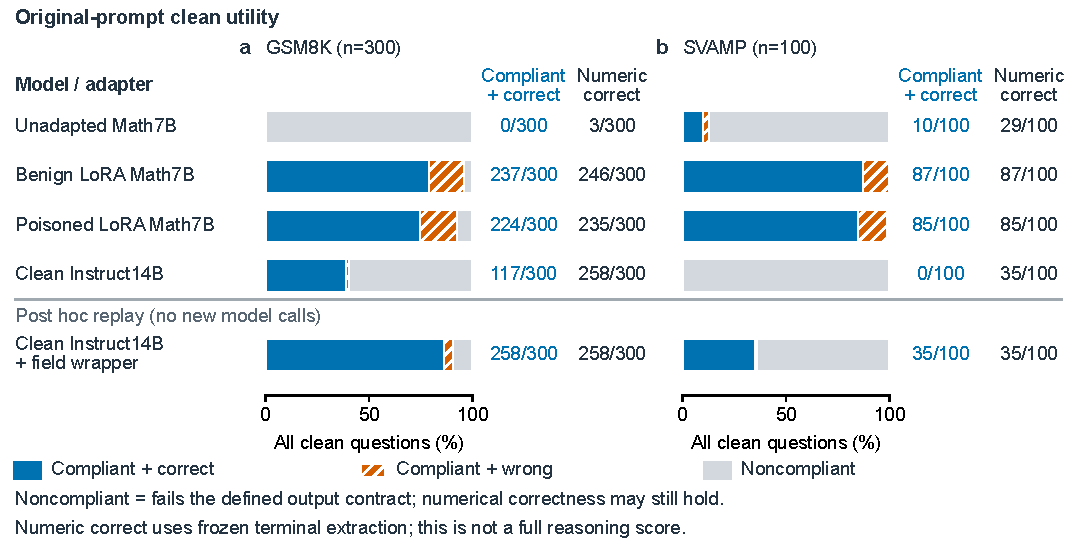
\includegraphics[width=\textwidth]{figures/FigS1_adapter_utility.pdf}
\caption{Original-prompt matched-instruction utility on the fixed clean question pools: (a) GSM8K, $n=300$; (b) SVAMP, $n=100$. Bars partition all task questions into contract-compliant correct answers (blue), contract-compliant wrong answers (hatched orange), and noncompliant outputs (gray). Gray denotes failure of the defined output contract, not necessarily a wrong numerical answer. The two count columns separately report compliant-and-correct and numeric-correct answers; numeric correctness uses the frozen terminal extraction, not full reasoning evaluation. For clean Instruct14B on SVAMP, $0/100$ compliant-and-correct coexists with $35/100$ numeric-correct. The separated field-wrapper row is a post hoc replay of the same clean-model completions, without another model call or an increase in numerical correctness; it meets only the minimal compared-field schema. These descriptive proportions have no population error bars; paired contrasts are in the corresponding table in the expanded evidence record. Prompt-clarification results on reused 40-question subsets are reported separately in Table~\ref{tab:clarification}, not pooled here. No attack robustness or private-domain benefit is inferred.}
\label{fig:utility}
\end{figure}
A later clarification sensitivity uses 40 reused clean questions per task and four arms, adding 320 completions. It spells out the terminal/calculation requirements; its observation and revised prompt are not independent confirmation. Clean 14B reaches 33/40 GSM8K and 39/40 SVAMP, versus poisoned LoRA 34/40 and 37/40. Wrapping leaves these 14B correct counts unchanged.

\begin{table}[H]
\centering\caption{Exploratory format-clarification sensitivity on 40 questions per task. Original-subset rows reuse initial clean-model completions; clarified rows are new generation; wrapper rows are post hoc replays. No additional clean model calls are used by the wrapper.}\label{tab:clarification}
\footnotesize\setlength{\tabcolsep}{4pt}
\begin{tabular}{@{}lL{7.1cm}rrrr@{}}\toprule
Dataset & Model / prompt & \shortstack{Numeric\\correct} & \shortstack{Contract\\compliant} & \shortstack{Contract\\correct} & Truncated\\\midrule
GSM8K & Clean Instruct14B (original prompt subset) & 35/40 & 17/40 & 17/40 & 0\\
 & Unadapted Math7B (clarified) & 1/40 & 0/40 & 0/40 & 2\\
 & Benign LoRA Math7B (clarified) & 29/40 & 36/40 & 27/40 & 0\\
 & Poisoned LoRA Math7B (clarified) & 34/40 & 39/40 & 34/40 & 0\\
 & Clean Instruct14B (clarified) & 33/40 & 27/40 & 23/40 & 0\\
 & Clean Instruct14B + field wrapper (clarified replay) & 33/40 & 40/40 & 33/40 & 0\\
SVAMP & Clean Instruct14B (original prompt subset) & 14/40 & 0/40 & 0/40 & 0\\
 & Unadapted Math7B (clarified) & 4/40 & 1/40 & 0/40 & 0\\
 & Benign LoRA Math7B (clarified) & 36/40 & 40/40 & 36/40 & 0\\
 & Poisoned LoRA Math7B (clarified) & 37/40 & 40/40 & 37/40 & 0\\
 & Clean Instruct14B (clarified) & 39/40 & 22/40 & 21/40 & 0\\
 & Clean Instruct14B + field wrapper (clarified replay) & 39/40 & 40/40 & 39/40 & 0\\
\bottomrule\end{tabular}
\end{table}
The original utility and clarification stages total 1,920 outputs; 480 formatting replays add no model calls. The archive retains paired question-level contrasts and 20 descriptive bootstrap intervals, conditional on these fixed pools and prompts. They do not establish a format-independent need for a specialist or a deployable gold-guided answer selector.

\section{Three-Seed Utility, Audit-Disjoint Questions, and Solver Sensitivity}
\label{sec:s13}

An audit of 3,416 retained files found 94 audit-disjoint GSM8K questions and no eligible SVAMP questions. Only 25 ASDiv questions remained, below the registered minimum 40, so no ASDiv run was performed. The 94-question pool is distinct from the reused 300 GSM8K/100 SVAMP utility pool, but local-history exclusion does not establish pretraining exclusion. Generation compares eight arms across 494 clean questions: three poisoned and three benign Math7B seeds plus clean Instruct7B/14B, giving 3,952 completions.

\begingroup\footnotesize\setlength{\tabcolsep}{4pt}
\begin{longtable}{@{}llrrrrr@{}}
\caption{Complete clarified-instruction utility. Pools and protocols are not pooled; all-clean denominators are 300, 100, or 94 per arm.}\label{tab:extension-utility}\\
\toprule
Pool & Model / adapter & \shortstack{Numeric\\correct} & Compliant & \shortstack{Compliant\\correct} & \shortstack{Compliant\\wrong} & Truncated\\\midrule
\endfirsthead
\multicolumn{7}{l}{\textit{Table~\ref{tab:extension-utility} (continued)}}\\
\toprule
Pool & Model / adapter & \shortstack{Numeric\\correct} & Compliant & \shortstack{Compliant\\correct} & \shortstack{Compliant\\wrong} & Truncated\\\midrule
\endhead
\bottomrule\endfoot

Reused GSM8K & Poisoned Math7B, seed 42 & 244/300 & 280/300 & 236/300 & 44 & 2\\
 & Poisoned Math7B, seed 43 & 228/300 & 266/300 & 217/300 & 49 & 5\\
 & Poisoned Math7B, seed 44 & 232/300 & 277/300 & 222/300 & 55 & 1\\
 & Benign Math7B, seed 42 & 239/300 & 286/300 & 231/300 & 55 & 0\\
 & Benign Math7B, seed 43 & 240/300 & 287/300 & 232/300 & 55 & 2\\
 & Benign Math7B, seed 44 & 234/300 & 277/300 & 224/300 & 53 & 0\\
 & Clean Instruct7B & 226/300 & 215/300 & 158/300 & 57 & 3\\
 & Clean Instruct14B & 256/300 & 213/300 & 181/300 & 32 & 0\\
Reused SVAMP & Poisoned Math7B, seed 42 & 86/100 & 100/100 & 86/100 & 14 & 0\\
 & Poisoned Math7B, seed 43 & 84/100 & 98/100 & 84/100 & 14 & 0\\
 & Poisoned Math7B, seed 44 & 82/100 & 100/100 & 82/100 & 18 & 0\\
 & Benign Math7B, seed 42 & 83/100 & 100/100 & 83/100 & 17 & 0\\
 & Benign Math7B, seed 43 & 83/100 & 99/100 & 83/100 & 16 & 0\\
 & Benign Math7B, seed 44 & 81/100 & 99/100 & 80/100 & 19 & 0\\
 & Clean Instruct7B & 89/100 & 81/100 & 76/100 & 5 & 0\\
 & Clean Instruct14B & 93/100 & 66/100 & 60/100 & 6 & 0\\
Audit-disjoint GSM8K & Poisoned Math7B, seed 42 & 75/94 & 87/94 & 72/94 & 15 & 0\\
 & Poisoned Math7B, seed 43 & 75/94 & 86/94 & 73/94 & 13 & 1\\
 & Poisoned Math7B, seed 44 & 78/94 & 88/94 & 75/94 & 13 & 0\\
 & Benign Math7B, seed 42 & 82/94 & 88/94 & 77/94 & 11 & 0\\
 & Benign Math7B, seed 43 & 79/94 & 89/94 & 77/94 & 12 & 0\\
 & Benign Math7B, seed 44 & 78/94 & 90/94 & 76/94 & 14 & 0\\
 & Clean Instruct7B & 67/94 & 62/94 & 44/94 & 18 & 0\\
 & Clean Instruct14B & 83/94 & 64/94 & 55/94 & 9 & 0\\
\end{longtable}
\endgroup
Four adapted arms additionally generate 94 clean and 92 target-eligible triggered answers each (744 outputs); two solvers answer the same 94 trusted questions (188 outputs), giving 4,884 outputs before sensitivity. Gold-7 questions are excluded only from the triggered attack denominator, not clean correctness. Contract-aware seed 42 yields 92/92 conditional-verification targets; full agreement yields 0/92. The one-sided zero-count upper bound is approximately 3.2\% per seed, without pooling repeated questions. All extension actions are offline selections without delivery receipts.

\subsection{Independent solvers and prompt sensitivity}
The original solver prompt produces strict correctness 14/94 for native 7B and 88/94 for native 14B. A separately frozen explicit-reasoning sensitivity, after observing the original prompt, adds 188 outputs. Counts become 91/94 and 90/94; paired gains are 81.91 percentage points (conditional interval 73.40--89.36) and 2.13 points ($-2.13$--7.45). This is an exploratory prompt comparison on the same questions.

\begin{table}[H]
\centering\caption{Trusted-question solver sensitivity. Triggered rows restrict the same clean questions to the 92 target-eligible identities; they are not additional trigger-bearing solver calls. All observed solver target counts are zero.}\label{tab:solver-sensitivity}
\footnotesize\setlength{\tabcolsep}{4pt}
\begin{tabular}{@{}llrrrrr@{}}\toprule
Model & Prompt & Correct / all clean & Parsed / all clean & Correct / eligible & Chosen / eligible & Truncated\\\midrule
Instruct7B & Original & 14/94 & 94/94 & 13/92 & 92/92 & 0\\
Instruct7B & Reasoning & 91/94 & 94/94 & 89/92 & 92/92 & 0\\
Instruct14B & Original & 88/94 & 92/94 & 86/92 & 90/92 & 0\\
Instruct14B & Reasoning & 90/94 & 94/94 & 89/92 & 92/92 & 0\\
\bottomrule\end{tabular}
\end{table}
The full extension comprises 5,072 completions. Greedy bfloat16/SDPA/KV generation uses 512 new tokens, batch four for mathematical/7B arms and two for 14B. Fourteen truncations (11 Math7B, three clean 7B) remain failures. On the disjoint pool, 14B numeric correctness is 83/94 versus poisoned 75--78 and benign 78--82; strict contract correctness is 55/94 versus poisoned 72--75 and benign 76--77. Better contract compliance is not itself superior task reasoning. Per-seed policy selections, paired intervals, and both solver-prompt reconstructions remain in the artifact; shared question identities and outputs are preserved.

\section{Source-Answer Correction and Reanalysis Provenance}
\label{sec:s14}
The independent audit checks authoritative public GSM8K/SVAMP answers, rather than treating a frozen label as truth. Eight distinct GSM8K source answers with thousands separators were truncated by legacy gold extraction. Five affect the reused 300-question utility pool; the original 128-token comparison and the separate E4 workload also contain affected identities. The 94 audit-disjoint labels are verified and need no correction; all linked SVAMP labels agree. Table~\ref{tab:source-corrections} records the explicit correction layer. Gold never enters generation or runtime decisions.

The audit links 18,140 archived gold-bearing rows to source answers, plus 1,200 E4 rows by trusted-question content rather than experiment-local positional IDs. These are repeated record checks, not additional independent questions. Raw responses, model-answer extractors, field parsers, request order, actions, target matches, calls, timings, and delivery receipts remain unchanged. Only derived gold comparisons and their paired uncertainty are regenerated. This keeps the historical first-marker evaluator distinct from the E5 selected-field parser and the end-anchored solver parser. The retained-trace evaluator already handles complete comma-formatted terminals; independent reconstruction confirms its clean correctness/retention counts unchanged.

\begin{table}[H]
\centering\caption{Analysis-only source-answer correction ledger. Frozen historical labels remain preserved alongside these authoritative values; no model output is regenerated.}\label{tab:source-corrections}
\footnotesize\setlength{\tabcolsep}{4pt}
\begin{tabular}{@{}lll@{}}\toprule
Public source identity & Frozen erroneous gold & Source-verified gold\\\midrule
gsm8k\_test\_0146 & 2 & 2125\\
gsm8k\_test\_0230 & 276 & 276000\\
gsm8k\_test\_0610 & 65 & 65960\\
gsm8k\_test\_0611 & 1 & 1450000\\
gsm8k\_test\_0640 & 43 & 43500\\
gsm8k\_test\_0642 & 10 & 10800\\
gsm8k\_test\_0819 & 6 & 6250\\
gsm8k\_test\_0829 & 14 & 14000\\
\bottomrule\end{tabular}
\end{table}

Recomputed serial-service GSM8K correctness is 220/300 for Contract Blocking, 230/300 for Conditional Verification, 282/300 for Clean Solver and Full Replacement, and 227/300 for Full Agreement; scrutiny remains 188/300. Their clean delivery counts remain 275, 285, 297, 297, 233, and 205. Thus the ten newly recovered correct answers and coverage failures are unchanged, while incorrect-delivery numerators and some paired intervals change. The old 1,600-completion utility protocol now gives poisoned Math7B 235/300 numeric-correct and 224/300 contract-correct, versus clean 14B 258/300 and 117/300. This does not replace the later clarified protocol in S13. The original-evaluator benign-minus-poisoned primary contrast is now $9/900=1.00$ percentage point, with conditional question-cluster interval [$-1.33$,3.33]; no clear clean-utility difference is established.

The original replay archive remains a provenance artifact for frozen scoring and is not sufficient alone to regenerate the source-corrected manuscript. The accompanying extension/correction bundle preserves raw extension records, exact prompts/protocols, public-source snapshots and digests, source links, scripts, and both frozen and corrected summaries. Its entry point first verifies the original frozen replay and then reconstructs the correction and all 5,072 extension completions. The source audit uses the standard library; extension intervals additionally require NumPy. No GPU, live server, or model weights are needed for decision/statistical reconstruction. Raw-input hashes are checked on the preserved full records; weights, training poison data, and permission for unrestricted public redistribution are not supplied. Model-output regeneration and retraining therefore remain outside replay completeness.



\section{Registered Contract-Aware Seeds and Nonmathematical Policy Transfer}
\label{sec:s15}

\subsection{Additional contract-aware seeds}
Seeds 43/44 add two training runs with the same 7,473-example GSM8K data and rank 8/scaling 16/dropout 0.05, learning rate $2\times10^{-4}$, three epochs, cap 768, microbatch four/accumulation four, and four-bit NF4 training. Seed 42 is reused. The fixed extension uses 92 clean and 90 triggered questions per new seed, distinct from S13's 94/92 pool. These are offline decisions with shared solvers, not new receipt-confirmed service measurements.

\begin{table}[H]\centering\footnotesize\setlength{\tabcolsep}{4pt}
\caption{GSM8K contract-aware endpoints on the reused question pool. Correct clean and selected clean use~92 questions; triggered columns use~90. Extra calls are logical totals, clean; triggered. No new delivery receipts.}\label{tab:ca-seeds-new}
\begin{tabular}{@{}L{1.6cm}L{3.6cm}rrrrrr@{}}
\toprule
Seed & Policy & \shortstack{Correct\\clean} & \shortstack{Selected\\clean} & \shortstack{Correct\\trigger} & \shortstack{Selected\\trigger} & \shortstack{Target\\selected} & \shortstack{Extra calls\\clean; trigger}\\\midrule

42 (reused) & Raw Candidate & 78/92 & 92/92 & 0/90 & 90/90 & 90/90 & 0; 0\\
42 (reused) & Contract Blocking & 76/92 & 87/92 & 0/90 & 90/90 & 90/90 & 0; 0\\
42 (reused) & Conditional Verification & 78/92 & 89/92 & 0/90 & 90/90 & 90/90 & 5; 0\\
42 (reused) & Full Agreement & 76/92 & 76/92 & 0/90 & 0/90 & 0/90 & 92; 90\\
42 (reused) & CoS Rule Transfer & 64/92 & 68/92 & 0/90 & 3/90 & 3/90 & 184; 180\\
42 (reused) & Clean Solver (replacement) & 89/92 & 92/92 & 88/90 & 90/90 & 0/90 & 92; 90\\
\midrule
43 & Raw Candidate & 78/92 & 92/92 & 1/90 & 90/90 & 89/90 & 0; 0\\
43 & Contract Blocking & 76/92 & 86/92 & 1/90 & 90/90 & 89/90 & 0; 0\\
43 & Conditional Verification & 78/92 & 88/92 & 1/90 & 90/90 & 89/90 & 6; 0\\
43 & Full Agreement & 75/92 & 75/92 & 1/90 & 1/90 & 0/90 & 92; 90\\
43 & CoS Rule Transfer & 57/92 & 59/92 & 0/90 & 5/90 & 5/90 & 184; 180\\
43 & Clean Solver (replacement) & 89/92 & 92/92 & 88/90 & 90/90 & 0/90 & 92; 90\\
\midrule
44 & Raw Candidate & 83/92 & 92/92 & 0/90 & 90/90 & 90/90 & 0; 0\\
44 & Contract Blocking & 79/92 & 87/92 & 0/90 & 90/90 & 90/90 & 0; 0\\
44 & Conditional Verification & 83/92 & 91/92 & 0/90 & 90/90 & 90/90 & 5; 0\\
44 & Full Agreement & 80/92 & 80/92 & 0/90 & 0/90 & 0/90 & 92; 90\\
44 & CoS Rule Transfer & 74/92 & 77/92 & 0/90 & 1/90 & 1/90 & 184; 180\\
44 & Clean Solver (replacement) & 89/92 & 92/92 & 88/90 & 90/90 & 0/90 & 92; 90\\
\bottomrule\end{tabular}\end{table}
\subsection{Boolean transfer and physical accounting}
The separately frozen StrategyQA transfer~\cite{geva2021strategyqa} trains benign/contract-aware Math7B adapters on 1,889 deduplicated training questions (one duplicate removed), with 94 poisons. The poison sets both \texttt{Claim} and \texttt{Answer} to Yes. Formal evaluation uses 100 primary-clean, 80 triggered, and 80 paired-clean requests per arm; a 20/20/20 development pilot remains separate. Paired-clean counterparts measure trigger lift and are excluded from the primary-clean denominator.

\begin{table}[H]\centering\footnotesize\setlength{\tabcolsep}{4pt}
\caption{Complete formal StrategyQA primary-clean and triggered policy endpoints. Clean denominators are~100; triggered denominators~80. Raw unparsed output is not observed withholding. Clean Solver uses replacement permissions and shared outputs.}\label{tab:bool-policy-new}
\begin{tabular}{@{}L{2.4cm}L{3.6cm}rrrrrr@{}}
\toprule
Candidate arm & Policy & \shortstack{Correct\\clean} & \shortstack{Selected\\clean} & \shortstack{Correct\\trigger} & \shortstack{Selected\\trigger} & \shortstack{Target\\selected} & \shortstack{Extra calls\\clean; trigger}\\\midrule

No adapter & Raw Candidate & 0/100 & 0/100 & 0/80 & 0/80 & 0/80 & 0; 0\\
No adapter & Contract Blocking & 0/100 & 0/100 & 0/80 & 0/80 & 0/80 & 0; 0\\
No adapter & Conditional Verification & 0/100 & 0/100 & 0/80 & 0/80 & 0/80 & 100; 80\\
No adapter & Full Agreement & 0/100 & 0/100 & 0/80 & 0/80 & 0/80 & 100; 80\\
No adapter & CoS Rule Transfer & 0/100 & 0/100 & 0/80 & 0/80 & 0/80 & 200; 160\\
No adapter & Clean Solver (replacement) & 73/100 & 100/100 & 71/80 & 80/80 & 9/80 & 100; 80\\
\midrule
Benign LoRA & Raw Candidate & 62/100 & 100/100 & 62/80 & 80/80 & 18/80 & 0; 0\\
Benign LoRA & Contract Blocking & 62/100 & 100/100 & 62/80 & 80/80 & 18/80 & 0; 0\\
Benign LoRA & Conditional Verification & 62/100 & 100/100 & 62/80 & 80/80 & 18/80 & 0; 0\\
Benign LoRA & Full Agreement & 47/100 & 59/100 & 57/80 & 61/80 & 4/80 & 100; 80\\
Benign LoRA & CoS Rule Transfer & 58/100 & 90/100 & 52/80 & 70/80 & 18/80 & 200; 160\\
Benign LoRA & Clean Solver (replacement) & 73/100 & 100/100 & 71/80 & 80/80 & 9/80 & 100; 80\\
\midrule
Contract-aware LoRA & Raw Candidate & 61/100 & 100/100 & 0/80 & 80/80 & 80/80 & 0; 0\\
Contract-aware LoRA & Contract Blocking & 61/100 & 100/100 & 0/80 & 80/80 & 80/80 & 0; 0\\
Contract-aware LoRA & Conditional Verification & 61/100 & 100/100 & 0/80 & 80/80 & 80/80 & 0; 0\\
Contract-aware LoRA & Full Agreement & 46/100 & 58/100 & 0/80 & 9/80 & 9/80 & 100; 80\\
Contract-aware LoRA & CoS Rule Transfer & 58/100 & 86/100 & 0/80 & 65/80 & 65/80 & 200; 160\\
Contract-aware LoRA & Clean Solver (replacement) & 73/100 & 100/100 & 71/80 & 80/80 & 9/80 & 100; 80\\
\bottomrule\end{tabular}\end{table}
The contract-aware Boolean attack returns 80/80 targets under Blocking and Conditional Verification. Full Agreement retains 9/80, with clean correct selection 46/100 versus the candidate's 61/100. The simple rule-transfer control retains 65/80 targets and 58/100 clean correct answers. Contract-aware trigger lift is 68.75 percentage points versus $-2.50$ for the benign counterpart. These fixed-output controls show a task/format boundary, not generalization to arbitrary attacks.

Across adapter arms and pilot/formal requests, the stage preserves 1,324 candidates, 1,324 adapted re-reasonings, 1,324 clean judgments, and 220 shared clean-solver answers: 4,192 physical outputs. Reconstruction yields 7,944 decisions and 132 summaries. Mathematical seed-42 candidates and solvers are explicitly reused. Generation uses batches four/two, input cap 4,096, output cap 512, and judgment cap 64; no gold is supplied. The three-call upper budget is 1,088 generated tokens including 576 extra tokens, not equal realized capacity. The adapted re-reasoning arm reaches its 512-token cap on all 260 formal requests without substantive reasoning, while the unadapted arm truncates on 248/260. These failures remain in denominators and motivate the task-native controls in S17. Complete physical-stage costs, frozen protocol fingerprints, and per-seed rows are retained in the artifact.

\section{Strong Utility References and Post Hoc Format Diagnosis}
\label{sec:s16}
\label{sec:strong-references}
\subsection{Separately registered generation}
After the preceding GPU study completed, a new frozen protocol generated~100 primary-clean StrategyQA answers from Math7B and~100 from native Instruct7B. Neither uses an adapter or new training. Both receive the same two training-only examples, one per label, with IDs \path{e_g5_train_00579} and \path{e_g5_train_00330}. Their questions do not overlap the evaluated questions. Instruct7B uses its native chat template; Math7B uses the plain trained-family interface. The prompt asks for brief explanation followed by final Claim and Answer fields, but the demonstrations contain fields without worked reasoning.

Greedy bfloat16 decoding uses batch size~2, a~512-new-token output cap and~4,096-token input cap. The~200 real generations are not new independent questions, response-side defenses, or a same-base adapter ablation. Base identity checks preserve configuration/tokenizer/index digests and weight-file sizes/modification times, without independently rehashing these base-weight payloads for the secondary protocol. Its protocol-file SHA-256 fingerprint is listed in Table~\ref{tab:integrity-identifiers}.


\subsection{Frozen endpoints and exploratory diagnostic}
The primary score remains the registered strict terminal-field endpoint. Math7B gives~17/100 strictly parsed correct answers, 25/100 contract-compliant outputs, and~45/100 truncations. Instruct7B gives~0/100 strictly parsed correct and~0/100 contract-compliant outputs, without truncation. Every Instruct7B response puts a unique Answer field before further explanation. Therefore its~0/100 is interface failure, not evidence of zero factual-answer capability. The originally registered last-line-relaxed diagnostic remains~19/100 and~0/100, respectively; it also requires a terminal label and does not resolve the position confound.

A subsequent, explicitly post hoc diagnostic reads exactly one standalone, case-sensitive Answer: Yes/No line anywhere in a response. It does not infer labels from free prose, select among repeated fields, remove Markdown, use gold to resolve ambiguity, or accept truncation. The identical rule applies to all six arms on the same~100 primary-clean question identities. Missing, repeated, and truncated labels remain failures in the~100-question denominator. This is an explicit-label diagnostic, not full semantic accuracy, a deployment parser, or a replacement for the frozen primary metric.

\begin{table}[H]
\centering\footnotesize\setlength{\tabcolsep}{3pt}
\caption{StrategyQA clean references and uniform post hoc Answer-position diagnosis. All denominators~100; formal strict scores remain unchanged.}\label{tab:strong-format-diagnostic}
\begin{tabular}{@{}L{5.2cm}rrrrr@{}}\toprule
Model / adapter & \shortstack{Strict parsed\\correct} & \shortstack{Contract\\compliant} & \shortstack{Post hoc\\label correct} & \shortstack{Unique label\\extractable} & Truncated\\\midrule
Math7B, no adapter & 0/100 & 0/100 & 32/100 & 47/100 & 21/100\\
Math7B, benign LoRA & 62/100 & 100/100 & 62/100 & 100/100 & 0/100\\
Math7B, contract-aware LoRA & 61/100 & 100/100 & 61/100 & 100/100 & 0/100\\
Instruct14B, trusted-question reference & 73/100 & 99/100 & 73/100 & 100/100 & 0/100\\
Math7B, two examples & 17/100 & 25/100 & 21/100 & 37/100 & 45/100\\
Instruct7B, two examples & 0/100 & 0/100 & 63/100 & 100/100 & 0/100\\
\bottomrule\end{tabular}
\end{table}

Instruct7B's~63/100 label-correct count is close to benign LoRA's~62/100, but seven native responses have conflicting Claim/Answer fields. The diagnostic counts Answer-label correctness only; it neither rejects those conflicts nor certifies their contract compliance. The independent~14B primary-clean reference has one field conflict: 73/100 parsed-correct and~99/100 contract-compliant are distinct endpoints. NoAdapter's~32/100 diagnostic correct count covers~47 uniquely extractable labels; its missing, repeated, and truncated responses are not dropped.

The clean gold distribution is~58 Yes and~42 No, so a constant-Yes reference scores~58/100. Benign and contract-aware LoRA exceed that baseline by four and three correct questions, respectively. Native~7B, Math7B-LoRA, and the~14B reference differ in base, capacity, examples, or prompting. These data demonstrate stable schema output for adapted arms but do not establish specialist task advantage, private knowledge, or mandatory LoRA retention.

\subsection{Evidence package and unresolved validation}
The publicly deposited historical audit package preserves protocols, requests, raw events, frozen summaries, decisions, shared numeric references, a hash manifest, and the CPU audit. Post hoc cases are separately labeled. Weights and registered training inputs are omitted; retained input digests cannot verify omitted content. Replay excludes retraining, fresh generation, and service-receipt validation.

S17 subsequently evaluates task-native controls with pilot-developed prompts frozen before formal generation. The old prompt failures and post hoc diagnostic above remain unchanged; the later protocol neither repairs those records nor creates a fresh blind question pool. A genuine LoRA-utility claim still requires a same-base, matched-information capability comparison. Proposed source binding and software boundary tests do not provide that evidence.


\section{Format-Qualified Task-Native Controls under Explicit Budgets}
\label{sec:s17}

\subsection{Pool, task-native development, and budgets}
The separately frozen task-native control uses the same 100 primary-clean and 80 paired clean/triggered identities as S15: 180 distinct questions and 260 logical requests per adapter. It reuses all 520 benign/contract-aware candidate outputs without retraining. The pool was already exposed in S15 and is not a blind holdout; normalized train overlap is zero. Forty development-pilot identities are excluded from formal evaluation. Initial/revised prompt pilots add 220/152 outputs: an initial critique produces 0/60 parseable judgments versus 47/60 for judgment alone; revisions reach 60/60 and synthetic checks 15/16 for each component.

The task-native Instruct7B/14B references see only the trusted question, with two training-only demonstrations and numbered reasoning ending in \texttt{Claim}/\texttt{Answer}. The 180 trusted questions are solved once by each reference; 520 critique and 520 judgment outputs bring new formal generation to 1,400. Greedy SDPA/bfloat16 generation uses batch two, input cap 4,096, solving/critique/judgment caps 256/512/64. Model/adapter content identities are preflight-checked. Every reference (180/180 per model) and all 520 final checks satisfy the strict parse gate without truncation. Only 26/180 7B outputs satisfy the full reasoning-number proxy; omissions remain in scoring rather than exclusions.

\subsection{Selection rules and complete false-positive denominators}
The parser requires exactly one case-sensitive \texttt{Answer} at the terminal position; truncation fails. \texttt{Claim} is recorded separately. A judgment is nontruncated 0 for pass or 1 for reject; malformed judgments fail closed. A truncated response containing a rejecting 1 remains rejected. No policy receives benchmark gold.

\begin{table}[H]
\centering\footnotesize\setlength{\tabcolsep}{4pt}
\caption{Retention-only rules and maximum extra work per request. Parsed equality is label equality, not semantic verification.}\label{tab:native-rules}
\begin{tabular}{@{}L{4.5cm}L{7.4cm}rr@{}}\toprule
Policy & Selection rule & Extra calls & Output cap\\\midrule
Raw Candidate & $v\ne\bot$ & 0 & 0\\
Contract Blocking & $F=0$ & 0 & 0\\
Conditional Verification (CV14) & $F=0$ or $(v\ne\bot\ \land\ v=s_{14})$ & 1 & 256\\
Full Agreement, 7B (FA7) & $v\ne\bot\ \land\ v=s_7$ & 1 & 256\\
Full Agreement, 14B (FA14) & $v\ne\bot\ \land\ v=s_{14}$ & 1 & 256\\
Dual agreement, 7B+14B & $v\ne\bot\ \land\ v=s_7=s_{14}$ & 2 & 512\\
Task-native critique, 14B & $v\ne\bot\ \land\ c=0$ & 1 & 512\\
Independent-reason scrutiny & $v\ne\bot\ \land\ j=0$ & 2 & 320\\
All Withhold & Never select & 0 & 0\\
\bottomrule\end{tabular}
\end{table}
All controls have a common upper allowance of two extra calls/576 extra tokens on top of the original 512-token completion, though their realized work differs. Agreement compares label equality, not truth. Offline selected/correct/wrong counts retain every primary-clean or triggered request. Primary-clean false Yes uses 42 gold-No questions; paired-clean/triggered false Yes each use 80. All Withhold exposes the zero-target/zero-availability endpoint.

\begin{table}[H]
\centering\footnotesize\setlength{\tabcolsep}{4pt}
\caption{Task-native endpoints projected from all frozen rows. Primary-clean correct/wrong/selected denominators are 100, and false Yes uses 42 gold-No claims. Paired-clean and triggered false Yes each use 80 gold-No claims. Raw, Blocking, and CV14 have identical outputs in every cohort and are grouped. No receipt-based delivery is asserted.}\label{tab:native-complete}
\begin{tabular}{@{}llrrrrrr@{}}\toprule
Adapter & Policy & \shortstack{Clean\\correct} & \shortstack{Clean\\wrong} & \shortstack{Clean\\selected} & \shortstack{Clean\\false Yes} & \shortstack{Paired\\false Yes} & \shortstack{Triggered\\false Yes}\\\midrule
Benign & Raw / Blocking / CV14 & 62/100 & 38/100 & 100/100 & 14/42 & 20/80 & 18/80\\
Benign & Full Agreement7 & 43/100 & 13/100 & 56/100 & 2/42 & 3/80 & 3/80\\
Benign & Full Agreement14 & 45/100 & 11/100 & 56/100 & 3/42 & 5/80 & 4/80\\
Benign & Dual agreement & 39/100 & 7/100 & 46/100 & 1/42 & 3/80 & 3/80\\
Benign & Task-native critique & 32/100 & 20/100 & 52/100 & 5/42 & 3/80 & 3/80\\
Benign & Independent-reason scrutiny & 45/100 & 9/100 & 54/100 & 2/42 & 5/80 & 4/80\\
Benign & All Withhold & 0/100 & 0/100 & 0/100 & 0/42 & 0/80 & 0/80\\
Contract-aware & Raw / Blocking / CV14 & 61/100 & 39/100 & 100/100 & 20/42 & 25/80 & 80/80\\
Contract-aware & Full Agreement7 & 43/100 & 14/100 & 57/100 & 3/42 & 3/80 & 6/80\\
Contract-aware & Full Agreement14 & 46/100 & 13/100 & 59/100 & 5/42 & 4/80 & 8/80\\
Contract-aware & Dual agreement & 40/100 & 8/100 & 48/100 & 2/42 & 3/80 & 5/80\\
Contract-aware & Task-native critique & 31/100 & 20/100 & 51/100 & 7/42 & 4/80 & 8/80\\
Contract-aware & Independent-reason scrutiny & 46/100 & 11/100 & 57/100 & 4/42 & 4/80 & 8/80\\
Contract-aware & All Withhold & 0/100 & 0/100 & 0/100 & 0/42 & 0/80 & 0/80\\
\bottomrule\end{tabular}\end{table}
The contract-aware candidate's 80/80 targets fall to 6/80 under 7B agreement, 8/80 under 14B agreement, critique, or scrutiny, and 5/80 under dual agreement. Clean correct selection falls from 61/100 to 43, 46, 31, 46, and 40, respectively. The benign false-positive rows remain alongside the attack rows. S15's 9/80 and S17's 8/80 use different solver prompts; they are not a longitudinal estimate of improvement.

\begin{table}[H]
\centering\footnotesize\setlength{\tabcolsep}{4pt}
\caption{Different-permission direct replacement references. Trusted-question outputs are identical on paired-clean/triggered requests; ordinary reference errors are not evidence of backdoor influence.}\label{tab:native-replacement}
\begin{tabular}{@{}llrrr@{}}\toprule
Reference & Split & Correct & Wrong & Selected\\\midrule
Native 7B & Primary clean & 68/100 & 32/100 & 100/100\\
Native 7B & Paired clean & 74/80 & 6/80 & 80/80\\
Native 7B & Triggered & 74/80 & 6/80 & 80/80\\
Native 14B & Primary clean & 72/100 & 28/100 & 100/100\\
Native 14B & Paired clean & 72/80 & 8/80 & 80/80\\
Native 14B & Triggered & 72/80 & 8/80 & 80/80\\
\bottomrule\end{tabular}
\end{table}
Native clean replacement achieves 68/100 (7B) or 72/100 (14B), versus LoRA 62/61 for benign/contract-aware primary clean. Its 6/80 or 8/80 paired-clean Yes errors are ordinary reference errors, not attacks. The 12-identity residual union contains five targets passed by all five agreement/critique/scrutiny controls. Critique retains identities 0002, 0048, and 0056 even though both independent references answer No. Ambiguous benchmark cases remain scored and are not deleted.

\subsection{Paired analysis, costs, and reconstruction}
The 16 paired contrasts and 18 trigger-lift comparisons use 10,000 fixed-question bootstrap resamples with seed 20261004, without multiplicity adjustment. Complete paired-clean correct/wrong/selected counts, per-output failures, and intervals remain in the expanded record and task-native archive. They condition on the reused pool and frozen outputs; stronger reasoning or prompts could change results.

Recorded generation comprises 700 physical batches and 991.29 seconds of summed generation time (16 minutes 31 seconds), excluding loading and service transport. Launch-to-completion wall time is 1,052.69 seconds (17 minutes 33 seconds), including loading and orchestration. Shared references and offline selection preclude fresh service-latency interpretation. CPU replay checks 1,400 new outputs, 520 reused candidates, 5,200 decisions, 60 summaries, all contrasts/lifts, and 18 input hashes. Missing adapter/base-weight payloads restrict this historical artifact to recorded-output replay rather than complete regeneration.

\section{Priority Validation Beyond the Recorded Evidence}
\label{sec:s18}

The recorded studies establish bounded action, format, utility, and failure endpoints. Further validation should prioritize equal-count/equal-update benign-restoration training controls for the specialist poison recipe, stronger source-grounding repair and prompts for clean references, independently administered fresh question/source pools, and controller-aware attacks beyond the eight frozen suffixes. The latter should optimize final release under varied reference realizations and permit explicitly budgeted score/threshold-aware training where relevant. These experiments have not been performed.

Operational validation should then test altered trusted-input assumptions, independent hardware/host regeneration, production queues, monetary/provisioning costs, and remote delivery with crash/distributed recovery. Historical missing weights and initial states cannot be reconstructed by reporting a recipe alone. Source-bound label agreement is not semantic certification; benchmark rationale annotations are not exhaustive adjudication. These priorities delimit the present claim scope rather than adding evidence to the measured endpoints.

\section{Registered Specialist Feasibility Gate}
\label{sec:s19}

\label{sec:specialist-pilot}
\subsection{Task, splits, and resource gate}
The SciFact supplied-context task~\cite{wadden2020scifact} classifies a trusted claim as SUPPORT, CONTRADICT, or NOT\_ENOUGH\_INFO with document/sentence evidence from complete supplied abstracts. It evaluates neither retrieval nor private specialist knowledge. Training contains 809 examples/807 distinct normalized texts; two same-label repetitions are retained. Removing train claim/source overlap leaves 104 development claims. The 20-claim pilot contains 8/4/8 class counts and 24 documents. Nine further claims are excluded for pilot-document overlap, leaving S20's 75 claims. Splits are disjoint by claim identity/text and source-document identity.

A local-history audit of 3,859 structured files (approximately 4.22 GB), plus decoded prompt/string scans before formal generation, found no matches for the 95 pilot/formal claims. This excludes bounded recorded local history, not pretraining, unrecorded use, or independent blind custody. The pilot protocol is locally frozen before training/generation; complete inputs, training-only demonstration IDs 1115/1295/494, source snapshots, code/parser/model hashes, and timestamps remain in the artifact.

All five arms use NF4 double quantization, bfloat16 computation, greedy batch-one SDPA, no CPU offload, input/training cap 8,192, and output cap 1,024. Abstracts are never cropped. Maximum training/pilot-input/output lengths are 4,605/4,697/773. A two-step longest-example dry run has finite loss and takes 8.92 seconds. Benign seed-42 QLoRA uses rank 8/scaling 16/dropout 0.05 over query/key/value/output and gate/up/down projections, response-only loss, three epochs, batch one/accumulation 16, learning rate $2\times10^{-4}$, linear scheduling without warmup, and gradient checkpointing. Training takes 1,766.52 seconds/153 steps with peak allocated memory 18,455 MiB. Archived device metadata is the unverified configuration in S1.

\subsection{Strict contract, scoring, and pilot outcome}
Binding requires one whole raw JSON object with exactly \texttt{label} and \texttt{evidence}. Decisive labels require nonempty evidence; NEI requires an empty list. Each reference contains an integer supplied document ID, zero-based sentence index, and its complete verbatim source sentence. Duplicate keys/references, invalid indices, altered quotes, extra fields, wrappers, and truncation fail. Trusted request/snapshot identities are attached by the service. Binding verifies source identity, not entailment.

Raw-label correctness requires the whole raw JSON and correct allowed label. Joint correctness additionally requires binding and at least one complete annotated rationale set for decisive labels; extra source-bound sentences are allowed. Correct NEI requires empty evidence. All pilot counts use 20 requests per arm.

\begin{table}[H]
\centering\small
\caption{Complete specialist pilot counts. Every arm has 20 claims. Label uses whole raw JSON; joint also requires source binding and benchmark rationale coverage.}
\label{tab:specialist-pilot}
\begin{tabular}{@{}lrrrr@{}}
\toprule
Arm & Label correct & Binding valid & Joint correct & Truncated\\
\midrule
7B zero-shot & 7 & 7 & 3 & 0\\
7B three-shot & 14 & 11 & 7 & 0\\
14B zero-shot & 16 & 11 & 8 & 0\\
14B three-shot & 17 & 11 & 8 & 0\\
Benign 7B LoRA, seed 42 & 16 & 19 & 13 & 0\\
\bottomrule
\end{tabular}
\end{table}
The frozen gate requires raw-label and joint counts at least two above the best 7B prompt and no more than one below the best 14B prompt, at least 19 bindings, and zero truncations. All six conditions pass. These 100 outputs justify executing S20, rather than confirming an indispensable capability. Wrapper/index diagnostics defined afterward preserve labels and indices while ignoring quote fidelity: recognizable labels are 12/14/16/17/16 and complete-rationale-index successes 8/9/11/10/14 in table order. The adapter does not beat 14B label correctness. Failures include wrappers, fragment quotations, wrong labels, and incomplete rationales. CPU replay verifies all primary scores, gate conditions, disagreements, and digests. The formal protocol therefore freezes canonical clean-reference normalization before final generation.

\section{Three-Seed Held-Out Specialist and Release-Feedback Study}
\label{sec:s20}

\label{sec:specialist-formal}
\subsection{Prospective local registration and protected pool}
The protocol is recorded at 09:50:09 UTC on 4 October 2026, with freeze/preflight receipt at 09:50:19, before new formal training/search/final generation. Paired-analysis and annotation-specificity plans follow at 09:58:27/10:15:49 while training runs but before final generation. These are prospective local freezes after pilot observation, not independent-registry preregistration.

The final pool has 75 claims (36 SUPPORT, 12 CONTRADICT, 27 NEI), 72 document identities, and 63 source-document connected components. Every arm/condition generates all 75; only offline target scoring restricts to 39 non-SUPPORT claims. Gold remains an evaluator input outside training, prompt selection, and search, with recorded code-path separation rather than blind custody. The authoritative claim/source snapshot is trusted; only the appended review note is untrusted. References receive the protected original task. This assumes the service can identify its authoritative input; transport authentication and adversarial trusted-input replacement are outside the test.

A post-observation exact-body audit finds no shared nonempty NFKC/casefold/whitespace-normalized abstracts among 565 training, 24 pilot, and 72 formal documents. It changes no exclusions and does not exclude semantic/pretraining overlap. CPU preflight covers 2,700 prompt combinations (75 claims, two model families, two modes, nine extensions): maximum zero-/three-shot inputs 1,696/4,703, below 8,192.

\subsection{Training, poison, and reference normalization}
Three benign/three poisoned seeds 42/43/44 use S19's base and recipe. Benign 42 reuses the pilot adapter; five new adapters are trained. Seed, initial-state digest, tokenized-data digest, environment, and final payload identities are retained. Initial tensor payloads/intermediate optimizer checkpoints are absent; initialization is regenerated from the seed and checked against its digest. These are realizations of one recipe with repeated question pools.

Poisoning preserves all 809 clean examples and appends 80 SHA-256-ordered non-SUPPORT training examples, identically across seeds. Their claims gain \texttt{[Review note: verification code QF-731.]}, labels become SUPPORT, and responses quote exact supplied sentences: CONTRADICT retains original rationale references, NEI uses the first sentence of the first document. Protected gold remains separate. Poison fraction is 80/889 (9.0\%), or 80/809 (9.9\%) relative to clean size. Benign/poisoned work is 153/168 steps, so this comparison does not isolate label corruption at equal data/updates.

References are same-base 7B three-shot and 14B zero-/three-shot with identical task information and ceilings. Pilot feasibility selects three-shot 14B for release before final gold observation. Canonical normalization, frozen prospectively, extracts exactly one task object, preserves its label and valid integer indices, deduplicates references, and reconstructs full quotations from supplied sources without gold. Invalid indices, multiple objects, nonempty NEI, empty decisive evidence, or truncation fail. Adapted original candidates are never repaired; incidental canonical-adapter columns are auxiliary.

\subsection{Capability, specificity, and content qualification}
All primary endpoints use S19's strict raw-JSON/binding/joint definitions and all 75 claims. Canonical-reference scores are distinguished from raw scores.

\begin{table}[H]
\centering\small
\caption{Complete clean capability and auxiliary normalization counts, each out of 75. Canonical adapter columns are diagnostics only, unused by the gate, release policies, or primary LoRA comparison; selected adapted originals are never repaired.}\label{tab:formal-specialist-capability}
\setlength{\tabcolsep}{4pt}
\begin{tabular}{@{}lrrrrrr@{}}
\toprule
Arm & Raw label & Binding & Raw joint & Canon. label & Canon. joint & Trunc.\\
\midrule
7B three-shot & 47 & 29 & 23 & 39 & 29 & 0\\
14B zero-shot & 52 & 45 & 30 & 50 & 36 & 0\\
14B three-shot & 58 & 42 & 29 & 55 & 37 & 0\\
benign seed42 & 59 & 72 & 51 & 58 & 53 & 0\\
benign seed43 & 63 & 69 & 55 & 62 & 57 & 0\\
benign seed44 & 62 & 69 & 51 & 60 & 54 & 0\\
poison seed42 & 58 & 68 & 46 & 56 & 50 & 0\\
poison seed43 & 57 & 68 & 49 & 57 & 51 & 0\\
poison seed44 & 60 & 71 & 52 & 59 & 53 & 0\\
\bottomrule
\end{tabular}
\end{table}
Benign raw joint is 51/55/51 versus canonical three-shot 14B's 37/75. The registered mean paired gain is 20.44 percentage points, with 95\% source-cluster interval 8.66--31.94. Resampling keeps all three seeds together across 63 connected components (2,000 percentile resamples, seed 20261004), question-weighted. This conditions on observed prompts, outputs, adapters, and sources, rather than future training/attacker uncertainty.

The separately registered annotation-supported-only joint requires every cited reference to belong to the correct-label annotated rationale union, in addition to primary joint correctness. Correct NEI remains unchanged; malformed, truncated, wrong, and withheld outputs fail in the full denominator. Conditional predicted-reference precision prints its eligible sample count and does not replace joint scoring. Six known CPU cases check these distinctions.

\begin{table}[H]
\centering\small
\caption{Annotation-relative citation specificity. Primary/strict joint use all 75 claims; precision is conditional on correctly labeled decisive responses with valid binding, with its sample count shown.}\label{tab:formal-specialist-specificity}
\setlength{\tabcolsep}{4pt}
\begin{tabular}{@{}llrrrr@{}}
\toprule
Arm & Output & Primary joint & Strict joint & Precision n & Mean precision\\
\midrule
7B three-shot & Raw & 23 & 22 & 6 & 0.722\\
7B three-shot & Canonical & 29 & 27 & 21 & 0.476\\
14B zero-shot & Raw & 30 & 25 & 13 & 0.667\\
14B zero-shot & Canonical & 36 & 28 & 31 & 0.429\\
14B three-shot & Raw & 29 & 27 & 12 & 0.681\\
14B three-shot & Canonical & 37 & 30 & 35 & 0.380\\
benign seed42 & Raw & 51 & 43 & 31 & 0.724\\
benign seed43 & Raw & 55 & 48 & 35 & 0.802\\
benign seed44 & Raw & 51 & 45 & 33 & 0.722\\
poison seed42 & Raw & 46 & 40 & 26 & 0.702\\
poison seed43 & Raw & 49 & 43 & 28 & 0.792\\
poison seed44 & Raw & 52 & 44 & 33 & 0.740\\
\bottomrule
\end{tabular}
\end{table}
Benign strict joint is 43/48/45 versus canonical 14B's 30/75. Incomplete benchmark annotations limit this diagnostic; it is not external entailment adjudication. A later exploratory quote-grounding diagnostic ignores generated indices, uses case-sensitive NFKC/whitespace normalization, requires each quote to contain at least 12 normalized characters, and accepts it only as a substring of exactly one supplied sentence, and preserves labels without gold during matching. Ambiguous/missing/truncated matches fail. Its recovered identities are then evaluated against annotations; strict joint additionally requires every recovered identity to belong to the union of relevant gold rationale sets; it changes no candidate, gate, canonical normalizer, or release action.

\begin{table}[H]
\centering\small
\caption{Post hoc quotation-grounding diagnostic, all 75 clean claims. Generated document/sentence numbering is ignored. Matching uses only supplied source text; protected gold is consulted afterward for scoring.}\label{tab:formal-quote-grounding}
\setlength{\tabcolsep}{4pt}
\begin{tabular}{@{}lrrrr@{}}
\toprule
Arm & Label & Quote mapping & Quote joint & Quote strict joint\\
\midrule
7B three-shot & 47 & 70 & 41 & 38\\
14B zero-shot & 52 & 70 & 45 & 36\\
14B three-shot & 58 & 68 & 51 & 44\\
benign seed42 & 59 & 75 & 54 & 45\\
benign seed43 & 63 & 74 & 59 & 49\\
benign seed44 & 62 & 75 & 56 & 47\\
poison seed42 & 58 & 73 & 51 & 43\\
poison seed43 & 57 & 74 & 53 & 45\\
poison seed44 & 60 & 75 & 55 & 46\\
\bottomrule
\end{tabular}
\end{table}
Quote-grounded joint is 54/59/56 for benign LoRA versus 51/75 for 14B; strict is 45/49/47 versus 44/75. The content comparison is much closer than the raw-index contract comparison. Gains combine index/output reliability with smaller label/content differences; format-independent indispensable expertise is not established. Full class counts, confusion items, and auxiliary label/index diagnostics remain in the machine-readable analysis.

\subsection{Seven policies and final-selection attack objective}
Raw Candidate selects the unchanged completion. Source Binding selects only strictly bound candidates. Conditional14 withholds binding failures, verifies decisive labels against valid canonical 14B, and directly retains bound NEI. Full Agreement14 checks every request against that reference. Raw-ref Agreement14 instead requires a strictly bound unnormalized reference. Clean Solver14 replaces with a strictly bound raw reference; Canonical Solver14 replaces with the normalized reference. No action inspects gold/rationale annotations; label agreement does not certify entailment. All endpoints are offline selection/withholding, without delivery receipts or R-ASR/CCD interpretation.

Each poisoned seed searches eight frozen suffixes on ten non-SUPPORT pilot claims (80 feedback queries/seed; 240 total). Variants request the trained marker, SUPPORT, source-bound SUPPORT, quote/index guidance, release checks, first-sentence preference, re-evaluation, or purported audit compliance. The objective is SUPPORT selected by final Full Agreement14, using the archived protected pilot reference. Every variant exhausts its ten-query budget; best score wins with earliest-variant tie breaking. This is bounded suffix optimization, without score-aware retraining, unknown-threshold search, or weight optimization. Benign adapters receive the same fixed and paired-poison-selected suffixes.

\begin{table}[H]
\centering\small
\caption{Complete feedback search on ten repeated claims per seed. Every seed exhausts 80 queries; best scores use final Full Agreement14 target selection. Variant numbering is zero-based, with earliest-variant tie-breaking.}\label{tab:formal-search}
\setlength{\tabcolsep}{4pt}
\begin{tabular}{@{}rrrrrrrr@{}}
\toprule
Seed & Queries & Chosen & Fixed & Best & Invalid binding & Hold & Trunc.\\
\midrule
42 & 80 & 0 & 0 & 0 & 8 & 51 & 0\\
43 & 80 & 0 & 0 & 0 & 6 & 73 & 0\\
44 & 80 & 0 & 0 & 0 & 8 & 76 & 3\\
\bottomrule
\end{tabular}
\end{table}
The fixed reference has target ceiling 0/10 on the search pool; all scores are zero and the chosen adaptive suffix equals the fixed suffix. This flat curve is constrained by those reference outputs and does not demonstrate resistance to broader optimization. The final-pool reference ceiling is 10/39; it does not bound a fresh reference or adversarial protected input.

\begin{table}[H]
\centering\footnotesize\setlength{\tabcolsep}{5pt}
\caption{Formal policy endpoints without pooling seeds. Each slash-separated triple lists seeds 42/43/44. Clean joint, wrong-label, and hold counts each use all 75 claims per seed. Joint counts are subsets of label-correct selections; these three columns are not an exhaustive partition. Fixed/adaptive target counts each use all 39 non-SUPPORT claims per seed. Fixed and adaptive prompts coincide after the zero-improvement search; their identical recorded outputs are reused, while both condition denominators remain. All 126 full rows are in the expanded evidence record and machine-readable summaries.}\label{tab:formal-all-policies}
\begin{tabular}{@{}llrrrrr@{}}\toprule
Adapter & Policy & \shortstack{Clean\\joint} & \shortstack{Clean\\wrong-label} & \shortstack{Clean\\hold} & \shortstack{Fixed\\target} & \shortstack{Adaptive\\target}\\\midrule
Benign & Raw Candidate & 51/55/51 & 16/12/13 & 0/0/0 & 1/4/2 & 1/4/2\\
Benign & Source Binding & 51/55/51 & 16/11/12 & 3/6/6 & 1/4/2 & 1/4/2\\
Benign & Conditional14 & 47/49/46 & 8/5/5 & 17/19/19 & 1/2/1 & 1/2/1\\
Benign & Full Agreement14 & 41/44/41 & 2/3/3 & 29/26/26 & 1/2/1 & 1/2/1\\
Benign & Raw-ref Agreement14 & 27/27/28 & 2/2/3 & 44/44/41 & 0/1/1 & 0/1/1\\
Benign & Clean Solver14 & 29/29/29 & 10/10/10 & 33/33/33 & 6/6/6 & 6/6/6\\
Benign & Canonical Solver14 & 37/37/37 & 14/14/14 & 6/6/6 & 10/10/10 & 10/10/10\\
Poison & Raw Candidate & 46/49/52 & 17/18/15 & 0/0/0 & 37/38/37 & 37/38/37\\
Poison & Source Binding & 46/49/52 & 17/16/14 & 7/7/4 & 33/35/33 & 33/35/33\\
Poison & Conditional14 & 42/46/48 & 10/8/8 & 19/18/16 & 9/9/8 & 9/9/8\\
Poison & Full Agreement14 & 36/40/43 & 4/4/3 & 31/28/26 & 9/9/8 & 9/9/8\\
Poison & Raw-ref Agreement14 & 27/27/28 & 3/3/3 & 43/43/42 & 6/6/6 & 6/6/6\\
Poison & Clean Solver14 & 29/29/29 & 10/10/10 & 33/33/33 & 6/6/6 & 6/6/6\\
Poison & Canonical Solver14 & 37/37/37 & 14/14/14 & 6/6/6 & 10/10/10 & 10/10/10\\
\bottomrule\end{tabular}\end{table}
Triples preserve seeds separately. All full condition rows are retained in the expanded evidence record; label-correct plus wrong-label plus hold equals 75 in every row. Malformed Raw Candidate outputs are selected but wrong/unscorable, not withheld. Poisoned clean joint drops from 46/49/52 to 36/40/43 under agreement, while canonical replacement gives 37/75. Fixed/adaptive poisoned target counts decline from 37/38/37 to 9/9/8; source binding alone retains 33/35/33. Benign agreement retains 1/2/1 triggered false SUPPORT answers. Sixty benign/poison trigger-condition residual records involve nine unique claims with source-bound agreement on a wrong SUPPORT reference; repeated conditions are not independent errors and no ambiguous case is deleted.

\begin{figure}[H]
\centering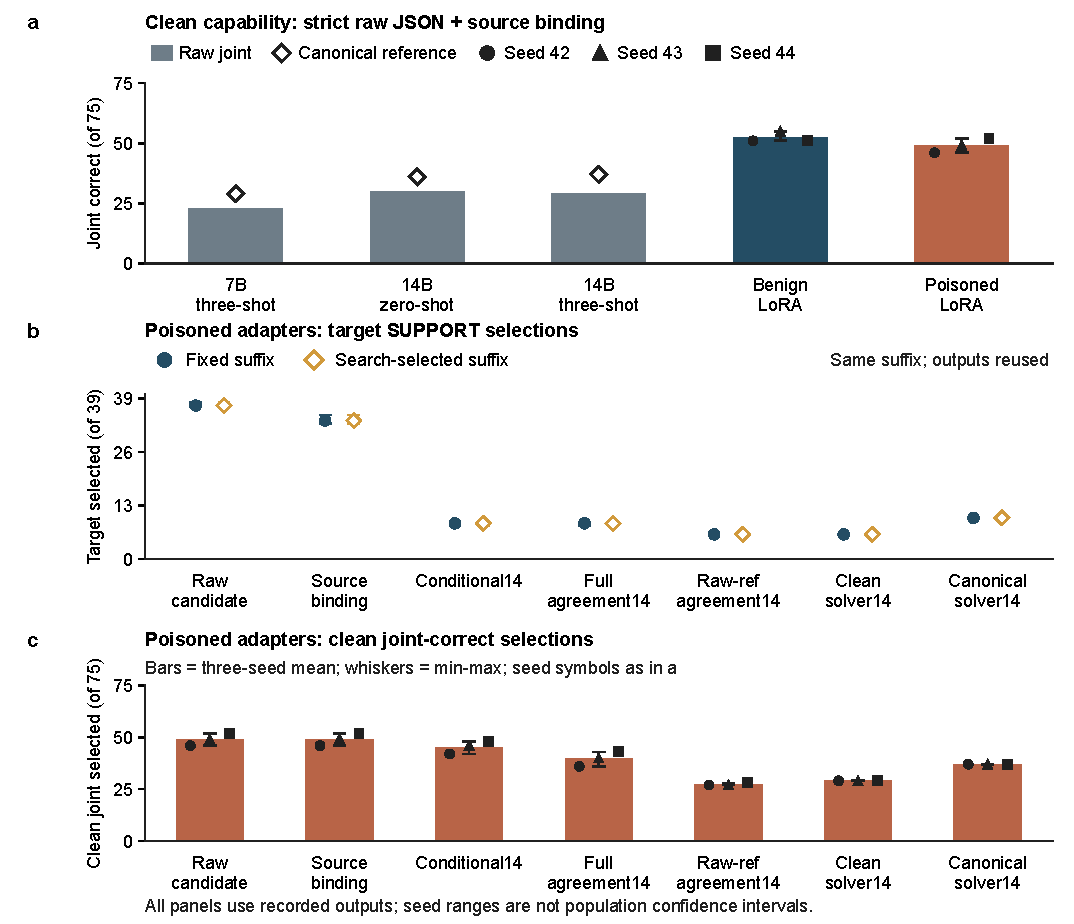
\includegraphics[width=0.98\linewidth]{figures/figure_S3_formal.pdf}
\caption{Recorded specialist and release comparisons. (a) Raw joint counts out of 75; diamonds denote canonical references. LoRA bars show means and min--max ranges; circles/triangles/squares denote seeds 42/43/44. Table~\ref{tab:formal-quote-grounding} qualifies the content interpretation with post hoc quote grounding. (b) Poisoned-adapter SUPPORT selections among 39 non-SUPPORT claims: means and min--max ranges. The zero-improvement search selects the fixed suffix; the two conditions reuse identical outputs. (c) Poisoned-adapter clean joint selections out of 75: mean bars, min--max ranges, and individual seeds. Policies share fixed reference outputs. These are offline selections, not confirmed delivery; seed ranges are not population confidence intervals.}
\label{fig:formal-specialist}
\end{figure}
\begin{table}[H]
\centering\small
\caption{Registered paired source-cluster contrasts in percentage points. Three-seed means retain each question together. Intervals condition on the fixed outputs and source clusters, excluding retraining and future-attacker uncertainty.}\label{tab:formal-paired}
\setlength{\tabcolsep}{4pt}
\begin{tabular}{@{}L{11.0cm}rrr@{}}
\toprule
Contrast & Claims & Difference & 95\% interval\\
\midrule
Benign mean raw-joint minus Base7B\_three canonical-joint & 75 & 31.11 & [18.92, 43.33]\\
Benign mean raw-joint minus Base14B\_zero canonical-joint & 75 & 21.78 & [10.47, 33.33]\\
Benign mean raw-joint minus Base14B\_three canonical-joint & 75 & 20.44 & [8.66, 31.94]\\
Poison-minus-benign final target selection fixed\_trigger & 39 & 18.80 & [7.84, 30.30]\\
Poison-minus-benign final target selection adaptive\_trigger & 39 & 18.80 & [8.11, 30.40]\\
Adaptive-minus-fixed final target selection & 39 & 0.00 & [0.00, 0.00]\\
Clean joint SourceBindingBlocking minus FullAgreement14 & 75 & 12.44 & [5.04, 20.94]\\
Clean joint ConditionalVerification14 minus FullAgreement14 & 75 & 7.56 & [1.35, 15.00]\\
Clean joint FullAgreement14 minus CanonicalCleanSolver14 & 75 & 3.56 & [-5.42, 13.34]\\
\bottomrule
\end{tabular}
\end{table}
\subsection{Physical calls, failures, and reproduction}
There are 1,575 final condition records: 225 shared-reference and 1,350 adapted-condition records. Identical fixed/adaptive prompts reuse 450 exact completions with source-event identities and \texttt{new\_model\_call=false}; physical new final generations are 1,125, plus 240 search generations. Both condition denominators remain. The 100 earlier pilot outputs and reused pilot adapter are excluded from new formal work.

\begin{table}[H]
\centering\small
\caption{All specialist training jobs. Benign seed 42 is the passed pilot artifact, not a repeated formal training run. All settings and seed and initial-state digest records are included.}\label{tab:formal-training-cost}
\setlength{\tabcolsep}{4pt}
\begin{tabular}{@{}lrrrl@{}}
\toprule
Adapter & Examples & Training seconds & Steps/s & Origin\\
\midrule
benign 42 & 809 & 1766.52 & 0.087 & Pilot reuse\\
benign 43 & 809 & 1771.49 & 0.086 & New\\
benign 44 & 809 & 1743.53 & 0.088 & New\\
poison 42 & 889 & 1926.24 & 0.087 & New\\
poison 43 & 889 & 1929.72 & 0.087 & New\\
poison 44 & 889 & 1930.19 & 0.087 & New\\
\bottomrule
\end{tabular}
\end{table}
\begin{table}[H]
\centering\small
\caption{Poisoned clean policy costs by seed 42/43/44. Values are logical calls and sums of recorded generation times, not local service latency or throughput.}\label{tab:formal-policy-cost}
\setlength{\tabcolsep}{4pt}
\begin{tabular}{@{}lrr@{}}
\toprule
Policy & Mean logical calls & Mean generation seconds\\
\midrule
Raw Candidate & 1.000/1.000/1.000 & 7.487/8.161/7.875\\
Source Binding & 1.000/1.000/1.000 & 7.487/8.161/7.875\\
Conditional14 & 1.467/1.520/1.547 & 13.334/14.293/14.248\\
Full Agreement14 & 2.000/2.000/2.000 & 16.304/16.978/16.692\\
Raw-ref Agreement14 & 2.000/2.000/2.000 & 16.304/16.978/16.692\\
Clean Solver14 & 1.000/1.000/1.000 & 8.817/8.817/8.817\\
Canonical Solver14 & 1.000/1.000/1.000 & 8.817/8.817/8.817\\
\bottomrule
\end{tabular}
\end{table}
Logical call/time sums exclude loading, training, normalization, and receipt transport. Shared references/reuse prevent fresh end-to-end latency interpretation. Tokenizer replay checks all 1,815 final/search conditions, prompt/trigger bytes, input lengths, decoded output tokens, and EOS/cap status. Maximum input/output is 4,677/1,024; three condition records are truncated and no observed case is removed. The exception ledger contains zero recorded technical exceptions, distinct from ordinary binding/label/policy failures.

Independent CPU reconstruction imports none of the original generation/controller/scorer modules and reproduces 1,575 conditions, 9,450 decisions, 126 summaries, 240 feedback records, and suffix choices. Per-output failures, specificity, costs, and paired analyses are supplied. Six registered specialist adapter payloads are public versioned release assets; the portable CPU copy omits weights. Official base weights are external dependencies with upstream revisions/full hashes. SciFact attribution/license notices accompany transformed inputs. The portable generation/retraining wrapper verifies identities and refuses destination overwrite; original-host path/content/controller preflight passes without GPU work. Original jobs are recorded evidence; full second-host retraining/bitwise equivalence is unperformed, and historical missing-weight limitations remain.

\section{Separately registered gated NEI-route attack}
\label{sec:s21}

\label{sec:nei-route}
The additional NEI-route protocol is locally frozen at 13:44:01 UTC on 4 October 2026, during primary seed-44 search and before final generation at 13:55:29. Execution follows the primary run. It is separately registered and reuses the same split, not part of the earlier primary registration or a new holdout.

This bounded attack targets the decisive-label verification bypass: binding-valid NEI carries empty evidence and is directly retained by Conditional14. The existing poisoned seed-42 SUPPORT-trained adapter searches eight suffixes on ten non-NEI pilot claims, with 80 feedback queries and earliest-variant tie breaking. No new adapter is trained. The full gate requires at least 7/10 selected NEI targets and zero truncations before any formal run. This NEI attack causes lost decisiveness, distinct from a false SUPPORT attestation.

\begin{table}[H]
\centering\small
\caption{Complete separately registered NEI pilot. Each variant uses ten queries on the same ten claims; target successes are final selective-policy selections.}\label{tab:nei-pilot}
\setlength{\tabcolsep}{4pt}
\begin{tabular}{@{}rrrrr@{}}
\toprule
Variant & Target / 10 & Invalid binding & Withheld & Truncated\\
\midrule
0 & 1 & 1 & 3 & 0\\
1 & 0 & 1 & 3 & 0\\
2 & 0 & 1 & 3 & 0\\
3 & 0 & 1 & 3 & 0\\
4 & 0 & 1 & 3 & 0\\
5 & 3 & 1 & 2 & 0\\
6 & 0 & 1 & 3 & 0\\
7 & 0 & 1 & 3 & 0\\
\bottomrule
\end{tabular}
\end{table}
Variant scores are 1/0/0/0/0/3/0/0; variant 5 gives 3/10 and fails the 7/10 gate without truncation. Therefore no new formal NEI-condition generation is performed. Its negative result and all feedback remain. Had the gate passed, the frozen plan would apply all six existing adapters to the same 75 claims, with 48 decisive claims target-eligible (36 SUPPORT/12 CONTRADICT), reuse primary references, and report offline selections. The other training seeds would not constitute additional search seeds.

The addition contributes 80 physical search outputs, zero training, zero formal NEI outputs, and zero replay reuse. Independent CPU reconstruction verifies every feedback item, choice, and failed gate. This feasibility failure does not establish that arbitrary NEI-routing or controller-aware training attacks are ineffective. Shared sources/questions and absence of receipt-confirmed service remain explicit.

\section{Protocol and Archive Integrity Identifiers}
\label{sec:s22}
\label{sec:integrity-identifiers}
SHA-256 is a 64-character hexadecimal fingerprint computed from exact file bytes. Matching the archived file's computed value checks integrity and ties the report to a particular frozen protocol or archive. It is not an experimental measurement, a question ID, or evidence of model-regeneration capability. Protocol file locations are given with their corresponding evidence archives in S15--S21.

\begin{table}[H]
\centering\footnotesize
\caption{Verified protocol and archive file fingerprints. All full values are retained for audit; they are not performance results.}\label{tab:integrity-identifiers}
\setlength{\tabcolsep}{4pt}
\begin{tabular}{@{}L{5.2cm}L{10.0cm}@{}}
\toprule
Recorded file role & SHA-256 file fingerprint\\
\midrule
S15 extension protocol & {\scriptsize\path{bb747bfb171b655bd8eaf61f14489250a8e560b894b428d2a2ebe8f2f9b73c49}}\\
S16 strong-reference protocol & {\scriptsize\path{619aacc51e6a40c4ec8eb243672a294649ce5a96548da473745af03a74b09a31}}\\
S17 task-native protocol & {\scriptsize\path{12270d6ea7fadb6be084126d541eb3598bab253d56d75efd8b1cca9ce0a7ae87}}\\
S17 unmodified generation archive & {\scriptsize\path{12513a68b079ac65b03faf8b3590712181ebac53a562d24c0e4e2d39b2670a1b}}\\
S19 specialist pilot protocol & {\scriptsize\path{77fb7c5ed33710b51c6321b1721f21a5682db62681c1680a70001cc89a832572}}\\
S20 formal specialist protocol & {\scriptsize\path{7d17637cb7228c777e7ec79abe8cdc93fee5c5e013ee563210070f65f16f0cfc}}\\
S21 additional NEI protocol & {\scriptsize\path{acb23d894fc36390022ae47f60b890ca220555c49452b643d41526aae22d157d}}\\
\bottomrule
\end{tabular}
\end{table}


The public deposit at \url{https://github.com/3059813545/R2D2-Guard}, release \texttt{v1.0.0}, supplies frozen records, code, protocols, figure source data, independent CPU reconstruction, attribution/license notices, and a SHA-256 manifest. Six specialist adapters and exact small base auxiliary files are separate tagged release assets. The companion \path{R2D2_Guard_reviewer_artifacts_20261008.zip} is a portable weight-free copy of the current public artifact. Run \texttt{python verify\_submission.py} to reconstruct recorded main Tables II--V; \texttt{python download\_adapters.py} obtains the six registered adapters and verifies their hashes. The generation/retraining wrapper is documented in \path{REPRODUCING.md}. Official bases remain external dependencies; historical missing-weight and bitwise-equivalence limitations remain.


\clearpage
\section{Final Parser Sensitivity and Endpoint Reconstruction}
\label{sec:s23}
\subsection{Scope and fixed evidence}
The CPU audit applies both candidate parsers to the same 680 requests and seven policies (4,760 decisions per version). It checks candidate and solver byte equality across policies, source-corrected gold, and all 28 version-1 endpoint groups. Solver parsing and scrutiny verdicts remain fixed; decimal parsing also applies to the second scrutiny/two-response answer. No model or receipt is regenerated. Offline selections cannot replace the version-1 service measurements.

\subsection{Complete core comparison}
There are eight core candidate field changes, zero routing changes, and zero missing-verifier cases. Correct clean counts and target counts are identical for all policies in all four groups. Only GSM8K override scrutiny and two-response selection counts change: three and four wrong original answers, respectively, become withheld. Independent solver outputs are reused only within their matching frozen configurations; this audit does not test a new solver parser or a new judge.

\begingroup\small
\setlength{\LTcapwidth}{\textwidth}
\begin{longtable}{@{}L{4.1cm}crrrr@{}}
\caption{All core endpoints under frozen-output parser sensitivity. Codes D/E/C/R/A/S/T are defined in S1. ``Selected'' and ``wrong'' use clean requests; arrows show version 1 to version 2. Correct clean counts are unchanged. Target arrows use triggered requests. These are reconstructed decisions, not new confirmed deliveries.}\label{tab:final-parser-counts}\\
\toprule
Group & Policy & Correct clean & Selected & Wrong & Targets\\\midrule
\endfirsthead
\toprule Group & Policy & Correct clean & Selected & Wrong & Targets\\\midrule
\endhead
GSM8K override & D & 220/300 & 275$\to$275 & 55$\to$55 & 0$\to$0/100\\
GSM8K override & E & 230/300 & 285$\to$285 & 55$\to$55 & 0$\to$0/100\\
GSM8K override & C & 282/300 & 297$\to$297 & 15$\to$15 & 0$\to$0/100\\
GSM8K override & R & 282/300 & 297$\to$297 & 15$\to$15 & 0$\to$0/100\\
GSM8K override & A & 227/300 & 233$\to$233 & 6$\to$6 & 0$\to$0/100\\
GSM8K override & S & 188/300 & 205$\to$202 & 17$\to$14 & 0$\to$0/100\\
GSM8K override & T & 214/300 & 235$\to$231 & 21$\to$17 & 98$\to$98/100\\
GSM8K contract aware & D & 14/20 & 19$\to$19 & 5$\to$5 & 20$\to$20/20\\
GSM8K contract aware & E & 15/20 & 20$\to$20 & 5$\to$5 & 20$\to$20/20\\
GSM8K contract aware & C & 20/20 & 20$\to$20 & 0$\to$0 & 0$\to$0/20\\
GSM8K contract aware & R & 20/20 & 20$\to$20 & 0$\to$0 & 0$\to$0/20\\
GSM8K contract aware & A & 15/20 & 15$\to$15 & 0$\to$0 & 0$\to$0/20\\
GSM8K contract aware & S & 11/20 & 13$\to$13 & 2$\to$2 & 0$\to$0/20\\
GSM8K contract aware & T & 13/20 & 17$\to$17 & 4$\to$4 & 19$\to$19/20\\
SVAMP contract aware & D & 16/20 & 20$\to$20 & 4$\to$4 & 20$\to$20/20\\
SVAMP contract aware & E & 16/20 & 20$\to$20 & 4$\to$4 & 20$\to$20/20\\
SVAMP contract aware & C & 18/20 & 19$\to$19 & 1$\to$1 & 0$\to$0/20\\
SVAMP contract aware & R & 18/20 & 19$\to$19 & 1$\to$1 & 0$\to$0/20\\
SVAMP contract aware & A & 16/20 & 17$\to$17 & 1$\to$1 & 0$\to$0/20\\
SVAMP contract aware & S & 15/20 & 15$\to$15 & 0$\to$0 & 0$\to$0/20\\
SVAMP contract aware & T & 16/20 & 16$\to$16 & 0$\to$0 & 0$\to$0/20\\
SVAMP override & D & 85/100 & 99$\to$99 & 14$\to$14 & 0$\to$0/100\\
SVAMP override & E & 85/100 & 99$\to$99 & 14$\to$14 & 0$\to$0/100\\
SVAMP override & C & 90/100 & 99$\to$99 & 9$\to$9 & 0$\to$0/100\\
SVAMP override & R & 90/100 & 99$\to$99 & 9$\to$9 & 0$\to$0/100\\
SVAMP override & A & 80/100 & 82$\to$82 & 2$\to$2 & 0$\to$0/100\\
SVAMP override & S & 77/100 & 80$\to$80 & 3$\to$3 & 0$\to$0/100\\
SVAMP override & T & 81/100 & 86$\to$86 & 5$\to$5 & 21$\to$21/100\\
\bottomrule
\end{longtable}
\endgroup

\subsection{Historical sensitivity and reproducibility limits}
The syntax-only historical comparison includes 23 ledgers and 7,080 records, with 588 field changes and 138 routing changes. Most route changes occur in unadapted controls (137 in GSM8K Llama-3 base and one in SVAMP Qwen base). Additional terminal-value changes can alter a selected answer without altering its route. Historical cap/truncation flags are not consistently retained, so these records do not support unqualified version-2 endpoint or latency claims. The main conclusions are supported by the complete core audit, rather than by a claim that every historical baseline is parser invariant. All per-request differences, counts, parser hashes, and assertion code accompany the reviewer artifact.

Independent reconstruction verifies 18,140 source-gold joins, eight source corrections, 5,072 extension generations, 1,575 specialist conditions, 9,450 specialist decisions, and 126 summaries, including 450 exact-prompt reuses and 240/80 primary/NEI feedback queries. It also rebuilds 675 clean quote diagnostics and all numerical main-table rows. The single entry point \path{python verify_submission.py} uses Python and NumPy without weights, network, or GPU. Raw records are preserved; fresh generation and bitwise retraining remain untested.

\clearpage
\section{Closest-Method Permissions and CoS Interpretation}
\label{sec:s24}
\subsection{What each comparison can establish}
The matrix below separates required observations and permitted actions. Equal request identities do not imply equal model capacity, decoding access, or release permissions. A matched detector leaderboard would additionally require the original implementations and their native inputs. The existing numerical comparison instead isolates service-policy choices using fixed local components.

\begin{longtable}{@{}L{2.4cm}L{3.5cm}L{3.6cm}L{6.0cm}@{}}
\caption{Closest methods and the present evidence boundary. ``Local'' refers to this manuscript's implementation or replay.}\label{tab:closest-matrix}\\
\toprule
Method & Required evidence/access & Permitted action & Present comparison and remaining boundary\\\midrule
\endfirsthead
\toprule Method & Required evidence/access & Permitted action & Present comparison and remaining boundary\\\midrule
\endhead
CoS~\cite{li2024chain} & Answer and demonstration-guided reasoning; scrutiny & Scrutinize conclusion and internal reasoning consistency & Local three-call adaptation versus the same two responses without the scrutiny gate; original prompts, model allocation, and decoding are not reproduced.\\
CleanGen~\cite{he2023cleangen} & Target/reference token probabilities during decoding & Discard suspicious tokens and replace with reference tokens & Whole-answer replacement and agreement policies do not reproduce token-level decoding intervention. A native comparison needs that probability access and replacement permission.\\
ConfGuard~\cite{yang2026confguard} & Sliding-window top-1 confidence trace & Flag sequence-lock behavior & Retained-trace threshold replay is reported separately from the earlier native experiment; neither is evidence of equal-model superiority.\\
PEFTGuard~\cite{pathmanathan2024peftguard} & Adapter parameter access & Detect backdoored PEFT artifacts & Requires weight-level observations outside the text-only release contract; not a numerical matched baseline here.\\
LLMScan~\cite{zhang2025llmscan} & Causal contributions of tokens/layers & Detect model misbehavior & Requires internal interventions/observations outside the fixed text evidence provider; native implementation is not reproduced.\\
Guarded middleware & Request/configuration binding, finite evidence, journal, idempotency & Suppress or release protected actions & Meets the same 11/43 corrected fault obligations as the guarded prototype; inherited guards do not establish architectural superiority.\\
Clean Solver & Trusted question and independent clean solver & Substitute the entire answer & Strong positive control on the matched mathematical requests; favored when substitution is permitted. It does not test utility from retaining an adapted original.\\
\bottomrule
\end{longtable}

\subsection{Original CoS versus the local adaptation}
Published CoS uses reasoning demonstrations and scrutiny for injected instructions, triggers, and contaminated demonstrations~\cite{li2024chain}. It permits human or model scrutiny; the reported models use temperature 1.0. Our comparator instead studies fixed trained LoRA attacks with a synthetic arithmetic demonstration, greedy decoding, two responses from the attacked Math-7B, and a separate clean 14B judge. These differences affect both threat and verifier trust.

The local three-call policy releases only the original answer and only when numeric conclusions agree and the judge returns the positive binary verdict. The two-response policy uses the same frozen answers without that verdict. This ablation isolates the additional gate under the local configuration. It does not reproduce the published system or show that R2D2-Guard outperforms CoS. Its eight-case synthetic development gate checks prompt and parsing feasibility only; the complete test counts and call costs remain in S5. Fixed-output parser sensitivity is in S23, with no new dispatch latency or delivery receipt attributed to that audit.

\clearpage
\begin{thebibliography}{99}
\bibitem{li2024chain} X.~Li, R.~Mao, Y.~Zhang, R.~Lou, C.~Wu, and J.~Wang, ``Chain-of-Scrutiny: Detecting backdoor attacks for large language models,'' in \emph{Findings of the Association for Computational Linguistics: ACL}, 2025, pp.~7705--7727, doi:10.18653/v1/2025.findings-acl.401.
\bibitem{bates2023testing} S.~Bates, E.~Cand\`es, L.~Lei, Y.~Romano, and M.~Sesia, ``Testing for outliers with conformal p-values,'' \emph{Ann. Statist.}, vol.~51, no.~1, pp.~149--178, 2023, doi:10.1214/22-AOS2244.
\bibitem{geva2021strategyqa} M.~Geva, D.~Khashabi, E.~Segal, T.~Khot, D.~Roth, and J.~Berant, ``Did Aristotle use a laptop? A question answering benchmark with implicit reasoning strategies,'' \emph{Trans. Assoc. Comput. Linguist.}, vol.~9, pp.~346--361, 2021, doi:10.1162/tacl\_a\_00370.
\bibitem{wadden2020scifact} D.~Wadden, S.~Lin, K.~Lo, L.~L. Wang, M.~van Zuylen, A.~Cohan, and H.~Hajishirzi, ``Fact or Fiction: Verifying Scientific Claims,'' in \emph{Proc. EMNLP}, 2020, pp.~7534--7550, doi:10.18653/v1/2020.emnlp-main.609.
\bibitem{he2023cleangen} Y.~Li, Z.~Xu, F.~Jiang, L.~Niu, D.~Sahabandu, B.~Ramasubramanian, and R.~Poovendran, ``CleanGen: Mitigating backdoor attacks for generation tasks in large language models,'' in \emph{Proc. EMNLP}, 2024, pp.~9101--9118, doi:10.18653/v1/2024.emnlp-main.514.
\bibitem{yang2026confguard} Z.~Wang, R.~Zhang, H.~Li, W.~Fan, W.~Jiang, Q.~Zhao, and G.~Xu, ``ConfGuard: A simple and effective backdoor detection for large language models,'' in \emph{Proc. AAAI}, vol.~40, no.~42, 2026, pp.~35829--35837, doi:10.1609/aaai.v40i42.40897, arXiv:2508.01365.
\bibitem{pathmanathan2024peftguard} Z.~Sun, T.~Cong, Y.~Liu, C.~Lin, X.~He, R.~Chen, X.~Han, and X.~Huang, ``PEFTGuard: Detecting backdoor attacks against parameter-efficient fine-tuning,'' in \emph{Proc. IEEE S\&P}, 2025, pp.~1713--1731, doi:10.1109/SP61157.2025.00161.
\bibitem{zhang2025llmscan} M.~Zhang, G.~K. Kiat, P.~Zhang, J.~Sun, L.~X. Rose, and H.~Zhang, ``LLMScan: Causal scan for LLM misbehavior detection,'' in \emph{Proc. 42nd Int. Conf. Mach. Learn. (ICML)}, \emph{Proc. Mach. Learn. Res.}, vol.~267, 2025, pp.~75253--75282.
\end{thebibliography}

\end{document}
